% Optimization Methods and Software submission
% Taylor & Francis Interact layout (reference style S)
% Ported from the Elsevier cas-sc manuscript (optimization_ready.tex).
\documentclass[]{interact}

\usepackage{epstopdf}% To incorporate .eps illustrations using PDFLaTeX, etc.
\usepackage[caption=false]{subfig}% Support for small, `sub' figures and tables

\usepackage[numbers,sort&compress]{natbib}% Citation support using natbib.sty
\bibpunct[, ]{[}{]}{,}{n}{,}{,}% Citation support using natbib.sty
\renewcommand\bibfont{\fontsize{10}{12}\selectfont}% Bibliography support using natbib.sty

% --- Packages carried over from the source manuscript ---
\usepackage{amssymb}
\usepackage{float}
\usepackage{algorithm}
\usepackage{multirow}
\usepackage{array}
\usepackage{longtable}
\usepackage{enumitem}
\graphicspath{{figures/}}
\restylefloat{figure}

% --- Theorem-like environments ---
\theoremstyle{plain}
\newtheorem{theorem}{Theorem}[section]
\newtheorem{lemma}[theorem]{Lemma}
\newtheorem{corollary}[theorem]{Corollary}
\newtheorem{proposition}[theorem]{Proposition}

\theoremstyle{definition}
\newtheorem{definition}[theorem]{Definition}
\newtheorem{example}[theorem]{Example}
\newtheorem{assumption}{Assumption}

\theoremstyle{remark}
\newtheorem{remark}{Remark}
\newtheorem{notation}{Notation}

% --- Author macros carried over from the source manuscript ---
\newcommand{\algstep}[1]{\smallskip\noindent\textbf{#1}}
\newcommand{\R}{\mathbb{R}}
\newcommand{\N}{\mathbb{N}}
\newcommand{\norm}[1]{\left\lVert #1 \right\rVert}
\newcommand{\abs}[1]{\left\lvert #1 \right\rvert}
\newcommand{\inner}[2]{\left\langle #1,\, #2 \right\rangle}
\DeclareMathOperator*{\argmin}{arg\,min}
\DeclareMathOperator*{\argmax}{arg\,max}
\DeclareMathOperator{\conv}{conv}
\DeclareMathOperator{\diag}{diag}
\DeclareMathOperator{\vecop}{vec}
\newcommand{\cvx}{\mathrm{cvx}}
\newcommand{\ps}{\mathrm{ps}}
\newcommand{\dtap}{\textsc{dtap}}

\begin{document}

\title{A Dual-Track Adaptive Projection Algorithm for a Nonlinear Split Feasibility Problem with Mixed Convex--Pseudoconvex Constraints}

\author{
\name{Nguyen Van The\textsuperscript{a}\thanks{Email: the.nv227153@sis.hust.edu.vn}, Tran Ngoc Thang\textsuperscript{a}\thanks{Email: thang.tranngoc@hust.edu.vn} and Nguyen Hong Son\textsuperscript{a}\thanks{CONTACT Nguyen Hong Son. Email: Son.NH240066D@sis.hust.edu.vn}}
\affil{\textsuperscript{a}Faculty of Mathematics and Informatics, Hanoi University of Science and Technology, No.~1 Dai Co Viet Street, Bach Mai Ward, Hanoi 100000, Vietnam}
}

\maketitle

\begin{abstract}
We study a nonlinear split feasibility problem whose output set is a normal box and whose component maps split into convex and pseudoconvex blocks. Classical $CQ$ solvers presuppose a linear operator, while existing self-adaptive methods require the aggregate proximity function to be convex, which a single pseudoconvex component invalidates. A Tchebyshev scalarization turns feasibility into a closed-form max-type violation function. We minimize it with the Dual-Track Adaptive Projection (\dtap) algorithm, which takes a residual-adaptive step on the convex constraints and a safeguarded diminishing step on the pseudoconvex ones, and projects each iterate onto the base set. Its step sizes need no operator-norm, Lipschitz, or Hölder modulus, yet we prove strong convergence to a feasible point. As an application, we recast two disjoint feature-selection models, one fractional-programming and one fuzzy-rough, as one nonlinear SFP, with no artificial terms; a sparse variant \dtap-S adds a feature budget. On eight UCI benchmarks \dtap{} matches or improves accuracy and AUC over the base models while reaching feasibility in fewer iterations, and \dtap-S yields compact, stable selections.
\end{abstract}

\begin{keywords}
Split feasibility problem; Pseudoconvex optimization; Tchebyshev scalarization; Adaptive (Lipschitz-free) step size; Strong convergence; Feature selection
\end{keywords}

\begin{amscode}
47J25; 90C25; 90C26; 65K05; 68T05
\end{amscode}

\section{Introduction}\label{sec:intro}

The \emph{split feasibility problem} (SFP), introduced by Censor and Elfving~\citep{censor1994}, seeks a point $x^\star\in C\subseteq\R^n$ whose image under a bounded linear operator $\mathcal{A}:\R^n\to\R^m$ lies in a convex set $Q\subseteq\R^m$:
\begin{equation}\label{eq:sfp-intro}
\text{find } x^\star\in C \quad\text{such that}\quad \mathcal{A}x^\star\in Q .
\end{equation}
It is a general formulation that specializes to convex feasibility, linear inverse problems, image reconstruction~\citep{byrne2002}, signal processing~\citep{combettes2011}, and radiotherapy planning~\citep{censor2006}. Its canonical solver is Byrne's $CQ$ method~\citep{byrne2002},
\begin{equation}\label{eq:cq-intro}
x^{k+1}=P_C\!\left(x^k-\tau\,\mathcal{A}^{\top}(I-P_Q)\mathcal{A}x^k\right),
\qquad \tau\in\bigl(0,\,2/\norm{\mathcal{A}}^2\bigr).
\end{equation}
This solver has two drawbacks, namely a step size depending on the operator norm $\norm{\mathcal{A}}$ and a projection $P_Q$ with no closed form for generic $Q$. The second is met by relaxed-projection variants~\citep{fukushima1986,yang2004}, which replace $Q$ by an outer half-space, and the first by the self-adaptive rule of L\'opez et al.~\citep{lopez2012}, which calibrates the step from the current value of the merit function $f(x):=\tfrac12\norm{(I-P_Q)\mathcal{A}x}^2$,
\begin{equation}\label{eq:lopez-intro}
\tau_n=\frac{\rho_n\,f(x_n)}{\norm{\nabla f(x_n)}^2},\qquad 0<\rho_n<4 .
\end{equation}
Rule~\eqref{eq:lopez-intro} is the reference point of this paper, so we isolate the mechanism behind it, beyond its removal of $\norm{\mathcal{A}}$. Its analysis turns on the single inequality $\inner{\nabla f(x)}{x-z}\ge 2f(x)$, valid at every solution $z$ because $I-P_Q$ is firmly nonexpansive; this inequality delivers both the admissible range $\rho_n\in(0,4)$ and the per-step decrease $\norm{x_{n+1}-z}^2\le\norm{x_n-z}^2-\rho_n(4-\rho_n)f^2(x_n)/\norm{\nabla f(x_n)}^2$. Strong convergence is available in Hilbert space through regularized and Krasnosel'ski\u{\i}--Mann variants~\citep{xu2010}. The mechanism above is therefore a property of the \emph{composition} $(I-P_Q)\mathcal{A}$: it comes from the linearity of $\mathcal{A}$, and the residual calibration alone does not provide it.

Linearity fails in many contemporary problems, among them the dose maps of intensity-modulated radiotherapy, where the differing densities of organs and tissues make the beam-to-dose relation nonlinear~\citep{li2013nsfp}, economic equilibrium models~\citep{yen2019}, and the training of neural predictors~\citep{tuan2024}. This leads to the \emph{nonlinear split feasibility problem} (NSFP): given closed convex $K\subseteq\R^n$ and $Q\subseteq\R^m$ and a nonlinear map $F:\R^n\to\R^m$,
\begin{equation}\label{eq:nsfp-intro}
\text{find } x^\star\in K \quad\text{such that}\quad F(x^\star)\in Q .
\end{equation}
The NSFP is not itself new. Li et al.~\citep{li2013nsfp} treat its multiple-sets form by minimizing a smooth Euclidean proximity function with a self-adaptive, backtracked step, while Yen et al.~\citep{yen2019} minimize the max-type merit $\max_i\lvert(I-P_{Q_i})F_i(x)\rvert^2$ over the solution set of an equilibrium problem, driving it by the Clarke subdifferential on the active index set, which is the same scalarization and active-set device we use below. Both papers replace, by a structural hypothesis, the quantitative inequality that linearity used to supply for free: \citep{li2013nsfp} require the aggregate proximity function to be convex, so that its gradient is co-coercive, and \citep{yen2019} require every component map to be \emph{quasilinear}, that is, both quasiconvex and quasiconcave. Neither hypothesis is ours, and neither of these classes coincides with the one we assume. Global convexity of the proximity function fails the moment a single component is only pseudoconvex; two-sided quasilinearity already excludes an ordinary convex map such as $x\mapsto x^2$, which is quasiconvex but not quasiconcave. We ask instead that each component be convex or pseudoconvex, a one-sided condition that these two classes neither contain nor are contained in, as Section~\ref{ssec:rel-nonlinear} makes precise. Two further difficulties attend the nonlinear case. When some $F_i$ is nonconvex the global gradient inequality is lost, so $CQ$-type separating hyperplanes may cut off the solution; and the available step sizes are tied either to a Lipschitz constant of $\nabla F$ or, for the wider quasi-convex class, to a H\"older modulus~\citep{hu2022quasi}, both hard to estimate at scale. Section~\ref{ssec:sfp-prelim} makes these challenges precise as (D1)--(D4). A complementary motivation comes from \emph{feature selection}~\citep{guyon2003,theng2024fs}, where embedded models cast selection as a constrained continuous program over a feature-weight vector. Two validated but isolated models live here: the fractional-programming model of Wang et al.~\citep{wang2021fractional}, which minimizes a redundancy-to-relevance ratio and is solved by a projection neural network, and the fuzzy-rough model AFRSFCV~\citep{wang2026afrsfcv}, which fuses class variance into fuzzy lower approximations and is solved by a softmax parametrization. Optimizing either in isolation tends to yield overly sparse selections, and neither offers a common language for combining criteria.

These two lines of work, nonlinear split feasibility on the one hand and embedded feature selection on the other, turn out to be two instances of a single problem. This paper addresses three questions.
\begin{enumerate}[label=\textbf{(Q\arabic*)},leftmargin=2.6em]
\item Is there a structured but broadly applicable subclass of NSFP for which one can design an iterative method that is simultaneously (i) free of operator-norm, Lipschitz, and H\"older constants; (ii) free of projections onto the intractable solution set; and (iii) provably \emph{strongly} convergent?
\item Can heterogeneous selection criteria, some convex and some only pseudoconvex, be expressed in one feasibility model \emph{without inventing new penalty terms}, so that the model inherits the empirical meaning of its constituents?
\item Does solving feature selection \emph{as} a feasibility problem offer any concrete advantage over solving each constituent model on its own, whether in selection quality, stability, or computational cost?
\end{enumerate}

We answer all three questions affirmatively. On the theoretical side we isolate the subclass of NSFP in which the output set is a \emph{normal box} $Q=(-\infty,b_1]\times\cdots\times(-\infty,b_m]$ and the component maps split into a convex group $I^{\cvx}$ and a pseudoconvex group $I^{\ps}$. The box structure admits a \emph{Tchebyshev scalarization}: measuring the residual in the sup-norm collapses $d_\infty(F(x),Q)$ into the closed-form max-type function $J(x)=\max_i (F_i(x)-b_i)^+$, which certifies feasibility one constraint at a time and whose maximizers expose the binding constraints. The split into convex and pseudoconvex groups then leads to a \emph{dual-track} step-size policy that reads exactly this information, described next.

We work in finite-dimensional Euclidean space with smooth component maps and a nonempty feasible set; these mild conditions are made precise in Assumption~\ref{ass:standing}. Our target is \emph{feasibility}, that is, returning a point of $\Omega$, rather than the minimization of a designated objective. Any optimization criterion of interest enters the model as one of the constraint functions $F_i$, so that `solving' the problem means bringing all criteria below their thresholds. This feasibility viewpoint allows several heterogeneous criteria, convex and pseudoconvex alike, to coexist in a single problem, and it lets a single algorithm with a single parameter setting serve the whole study. The price is that we do not claim optimality of the returned point for any one criterion; we return a point that is acceptable for all of them, which is the requirement in the feature-selection application.

This paper makes five principal contributions.
\begin{enumerate}[label=\textbf{C\arabic*.},leftmargin=2.4em,itemsep=4pt]
\item \textbf{A tractable nonlinear split-feasibility model.} We formulate the \emph{normal-box} NSFP with mixed convex--pseudoconvex components and derive, from a Tchebyshev scalarization, a closed-form max-type violation function $J$ whose zero set coincides with the feasible set. This turns an abstract feasibility requirement into a single nonsmooth merit function whose maximizers identify the binding constraints, which is the structure the dual-track step exploits (Section~\ref{sec:convergence}).
\item \textbf{The \dtap{} algorithm with Lipschitz-free adaptive steps.} We propose the Dual-Track Adaptive Projection algorithm, which decomposes the constraint index set into a convex track and a pseudoconvex track and assigns each the step rule that fits its geometry. On the convex track we extend rule~\eqref{eq:lopez-intro} to the nonlinear setting: the step is $\lambda\,\Phi^{\cvx}_k/\norm{g^{\cvx}_k}^2$ with $\lambda=2\rho_{\cvx}\in(0,4)$, where $\Phi^{\cvx}$ is a partial quadratic violation and $g^{\cvx}$ its gradient. Equivalently it is a Polyak step~\citep{polyak1969} for $\Phi^{\cvx}$ with known optimal value zero, but with the \emph{doubled} relaxation range of L\'opez et al.\ rather than the classical $(0,2)$; the doubling is no longer licensed by firm nonexpansiveness, which linearity would have supplied; it now rests on the aggregated inequality $\inner{g^{\cvx}_k}{x^k-x^\star}\ge2\Phi^{\cvx}_k$ that convexity of the individual $F_i$ still yields. On the pseudoconvex track, where only sign information remains, we use a \emph{safeguarded diminishing step}. The two directions are merged by a soft proportional weight, and each iteration ends with a single projection onto the base set $K$. No operator norm, Lipschitz, or H\"older constant is needed, and the method projects only onto the base set, never onto the output set $Q$ or the intractable solution set (Section~\ref{sec:convergence}).
\item \textbf{A strong-convergence theorem.} We prove that the \dtap{} iterates converge \emph{strongly} to a feasible point under three mild assumptions (Theorem~\ref{thm:strong}). The proof rests on a novel one-step quasi-Fej\'er inequality that yields boundedness, distance convergence, and decay of the convex-track violation; feasibility on the pseudoconvex track is then secured by a contradiction argument driven by continuity and pseudoconvexity. The purely convex and purely pseudoconvex regimes follow as corollaries, and a best-violation rate of $O(N^{-1/3})$ is obtained (Section~\ref{sec:convergence}).
\item \textbf{A unified, constraint-faithful feature-selection framework.} We show that the fractional-programming model~\citep{wang2021fractional} and the fuzzy-rough-set model AFRSFCV~\citep{wang2026afrsfcv} reduce to a \emph{single} normal-box NSFP whose three constraint functions are taken \emph{unchanged} from the two models' own objectives, namely two convex terms from the fuzzy-rough model and one pseudoconvex ratio from the fractional model. No artificial penalty is introduced, so the unified model preserves the empirical semantics of its constituents while becoming directly solvable by \dtap; new criteria can be appended simply as further convex or pseudoconvex constraints, and a sparse-projection variant \dtap-S adds an explicit, tunable feature budget (Section~\ref{sec:fs}).
\item \textbf{Empirical validation.} On eight UCI benchmarks spanning a wide range of sample sizes, dimensions, class counts, and balance levels, and against four baselines (the two base models and two subgradient variants for quasi-convex feasibility~\citep{hu2022quasi}), \dtap{} preserves or improves accuracy and AUC over the base models, with the gains concentrated on the SVM classifier and significant at the nominal level under Wilcoxon and Friedman tests, and it produces stable, consistent feature sets. Against the same-class subgradient methods \dtap{} yields nearly identical selections yet reaches feasibility in substantially fewer iterations and lower wall-clock time, up to three orders of magnitude on the larger datasets, while avoiding the H\"older-modulus estimation those methods require (Section~\ref{sec:experiments}).
\end{enumerate}

The paper is organized as follows. Section~\ref{sec:related} reviews the literature and positions \dtap{} against twelve representative prior works. Section~\ref{sec:prelim} collects the analytical preliminaries. Section~\ref{sec:convergence} states the normal-box NSFP, derives the Tchebyshev merit function, presents the dual-track decomposition and the standing assumptions, specifies \dtap, and then develops the convergence analysis. Section~\ref{sec:fs} builds the unified feature-selection framework. Section~\ref{sec:experiments} reports the numerical study, and Section~\ref{sec:conclusion} concludes with limitations and extensions.

\section{Related work}\label{sec:related}
We review four threads (linear split feasibility, nonlinear and quasi-convex feasibility,
optimization-based feature selection, and decomposition) and position \dtap{} in
Table~\ref{tab:related}.

\subsection{Linear split feasibility}\label{ssec:rel-linear}
Introduced by Censor and Elfving~\citep{censor1994}, the SFP was simplified by
Byrne's $CQ$ method~\citep{byrne2002}, which uses only $P_C,P_Q$ and a gradient step through
$\mathcal{A}^{\top}(I-P_Q)\mathcal{A}$ but pays with a step size tied to $\norm{\mathcal{A}}^2$
and a projection $P_Q$ explicit only for structured $Q$. Two lines address these costs:
relaxed-projection methods~\citep{fukushima1986,yang2004} replace $Q$ by an outer half-space with
closed-form projection, and the self-adaptive rule~\eqref{eq:lopez-intro} of L\'opez et
al.~\citep{lopez2012} calibrates the step from the current residual, removing
$\norm{\mathcal{A}}$. Xu~\citep{xu2010} proved \emph{strong} convergence for regularized and
Krasnosel'ski\u{\i}--Mann variants in Hilbert space.

Rule~\eqref{eq:lopez-intro} has since been extended beyond convex sets. Chen et
al.~\citep{chen2019ssub} keep it verbatim, as $\rho_k=\lambda_k f_k(u_k)/\norm{\nabla f_k(u_k)}^2$
over relaxed level sets $C_{k,\xi},Q_{k,\xi}$, and allow the level-set functions $c,q$ to be
continuous but nonconvex by replacing the subdifferential with an \emph{$S$-subdifferential}: a
modulus $r_f>0$ must exist for which $f+\tfrac{r_f}{2}d_S^2$ is subdifferentiable, equivalently
$\partial_{S,r_f}f(u)=\partial f(u)+r_f(I-P_S)(u)$. This is a genuine relaxation of convexity, but
it is neither ours nor comparable to ours: a pseudoconvex $F_j$ need not admit such an $r_f$, and a
function that does need not be pseudoconvex. What matters more for the present paper is where the
nonconvexity is placed. In~\citep{chen2019ssub} the operator remains a \emph{matrix}, so the merit
function $f_k(u)=\tfrac12\norm{\mathcal{A}u-P_{Q_{k,\xi}}\mathcal{A}u}^2$ is a convex composition
and the subgradient inequality that drives their proof is available for free; the nonconvexity
sits in the sets, never in the map. Their relaxation range is accordingly $\lambda_k\in(0,2)$,
obtained from the plain gradient inequality rather than from the co-coercivity that yields
L\'opez et al.'s $(0,4)$. The residual-based, constant-free philosophy of this thread and its
strong-convergence target inform our design; the mechanism that licenses it does not carry over to
a nonlinear $F$, and Section~\ref{ssec:rel-nonlinear} takes up what replaces it.

\subsection{Nonlinear and quasi-convex feasibility}\label{ssec:rel-nonlinear}
When the map is nonlinear, the global gradient inequality fails and $CQ$-type hyperplanes may
exclude the solution. The closest predecessor is Li et al.~\citep{li2013nsfp}, who pose the
nonlinear \emph{multiple-sets} SFP (find $x\in\bigcap_i C_i$ with $F(x)\in\bigcap_j Q_j$ for a
continuously differentiable $F$) and minimize over a bounded convex $\Omega\supseteq\bigcap_iC_i$
the Euclidean proximity function
$p(x)=\tfrac12\sum_i\alpha_i\norm{(I-P_{C_i})x}^2+\tfrac12\sum_j\beta_j\norm{(I-P_{Q_j})F(x)}^2$
by the projected step $x^{k+1}=P_\Omega[x^k-\beta_{k+1}\nabla p(x^k)]$, the step $\beta_{k+1}$
being chosen self-adaptively by backtracking. That framework does not sit beside our geometry; it
contains it. A normal box is the intersection $\bigcap_{i=1}^m\{z\in\R^m:z_i\le b_i\}$ of $m$
half-spaces, so with $C_1=K$ and the componentwise violation $v_i(x):=(F_i(x)-b_i)^+$ one has
$\norm{(I-P_{Q_i})F(x)}=v_i(x)$ and therefore
\begin{equation}\label{eq:li-reduction}
p(x)=\tfrac12\sum_{i=1}^m\beta_i\,v_i(x)^2,\qquad
\nabla p(x)=\sum_{i=1}^m\beta_i\,v_i(x)\,\nabla F_i(x).
\end{equation}
Comparing~\eqref{eq:li-reduction} with the \dtap{} direction~\eqref{eq:phi-g-cvx} below,
$g^{\cvx}$ is exactly $\nabla p$ with unit weights, restricted to the $\delta$-active convex
indices. The direction is therefore not where the novelty lies, and we do not claim it there; the novelty lies in what makes the step legitimate. The convergence proof of~\citep{li2013nsfp} runs entirely on
co-coercivity of $\nabla p$, which their Lemma~2.4 obtains from \emph{convexity of $p$} together
with a Lipschitz $\nabla p$ on the bounded $\Omega$; co-coercivity also keeps the
right-hand side of their backtracking test nonnegative, and hence makes the search terminate at
all. On a normal box, $p$ is convex precisely when every $F_i$ is convex, since then
$v_i=(F_i-b_i)^+$ is convex and nonnegative and $t\mapsto t^2$ is convex and increasing on
$[0,\infty)$. A single pseudoconvex component invalidates these implications: $v_j^2$ need not be convex, $p$ need not be convex, and $\nabla p$ need not be monotone, so the right-hand side of their backtracking test may become negative.\footnote{In the notation of Eq.~(3.3) of~\citep{li2013nsfp}, the acceptance test requires $\beta_{k+1}\norm{\nabla p(x^k)-\nabla p(x^{k+1})}^2\le(2-\mu)\inner{x^k-x^{k+1}}{\nabla p(x^k)-\nabla p(x^{k+1})}$; its right-hand side is nonnegative for every pair of iterates iff $\nabla p$ is monotone, which on a normal box holds iff every $F_i$ is convex.} When it does, no positive step size satisfies the test, and the line search is not well-defined. \dtap{} replaces the global and unverifiable
hypothesis `$p$ is convex' by a classification that can be checked one constraint at a time, and
replaces the search by a closed-form step; it also drops the requirements that $\Omega$ be bounded
and that $F,\nabla F$ be globally Lipschitz, deriving boundedness of the iterates instead
(Lemma~\ref{lem:bounded}).

The other close nonlinear predecessor is Yen et al.~\citep{yen2019}, and the overlap is at the
level of the merit function and its differentiation, not merely the topic. On a normal box their
componentwise term $p_i(x)=\lvert(I-P_{Q_i})F_i(x)\rvert^2$ equals $v_i(x)^2$ and their gradient
$\nabla p_i(x)=2(I-P_{Q_i})F_i(x)\nabla F_i(x)$ equals $2v_i(x)\nabla F_i(x)$, so their scalarized
objective $\max_i p_i$ is the square of our $J$ and their search direction, a convex combination
of active $\nabla p_i$ selected through the active set $I(x)=\{i:p_i(x)=p(x)\}$ and the Clarke
identity $\partial^0 p(x)=\mathrm{co}\{\nabla p_i(x):i\in I(x)\}$, is exactly the mechanism our
tracks~\eqref{eq:phi-g-cvx}--\eqref{eq:phi-g-ps} implement. We do not reintroduce that mechanism as
novel. Three differences separate the methods, and each is verifiable. First, the admissible map
class. Yen et al.\ require every $F_i$ to be \emph{quasilinear}; we require convex or
pseudoconvex. Neither class contains the other: $x\mapsto x^2$ is convex, hence covered here, but
not quasiconcave, hence excluded by their (A2); conversely a monotone cubic $x\mapsto x^3$ is
quasilinear, hence covered by them, but has a stationary point that is not a minimizer and so is
neither convex nor pseudoconvex. Second, the driving step. Their feasibility direction is a
normalized subgradient with a diminishing step $\alpha_k=\beta_k/\max\{\delta_k,\norm{g_k}\}$
under $\sum\beta_k^2<\infty$; on our convex track we instead use the residual-adaptive
rule~\eqref{eq:lopez-intro}, whose length is set by the current violation rather than by a
prescribed sequence, and which is not diminishing. Third, the source set. Their $C$ is the
solution set of a paramonotone equilibrium problem, handled by a second projected-subgradient
track, whereas ours is the explicit base set $K$; this is a deliberate modelling choice, since in
our target application $K$ is a simplex or box onto which projection is closed-form, and it lets
the second track address the \emph{pseudoconvex output constraints} rather than an implicit source
constraint. In short, Yen et al.\ decompose source-versus-image; \dtap{} decomposes the image
constraints by their individual geometry.

The remaining nonlinear thread is quasi-convex feasibility. Tuan et al.~\citep{tuan2024} embed
split-feasibility constraints in controllable Pareto-front learning, and Hu et
al.~\citep{hu2022quasi} solve systems of quasi-convex inequalities by subgradient methods with
constant and dynamic steps. Their constraint class is strictly \emph{larger} than ours: convex and
pseudoconvex functions are quasi-convex, so~\eqref{eq:nsfp-box} is one of their instances, and we
accordingly use their two variants as baselines in Section~\ref{sec:experiments}. This is the
opposite relation to the one with Yen et al.: Hu et al.\ sit outside and above our class, Yen et
al.\ beside it. Generality has a price. A uniform treatment of the whole quasi-convex class leaves
only sign information on every constraint, so their dynamic step must be calibrated by a H\"older
modulus that is large and unreliable on real data. \dtap{} does not enlarge the class; it exploits
the finer convex/pseudoconvex split \emph{inside} it to recover a quantitative gradient inequality
on part of the system, and with it a step that needs no modulus at all.


\subsection{Optimization-based feature selection}\label{ssec:rel-fs}
Two embedded, optimization-based models anchor our application (see the surveys
\citep{guyon2003,theng2024fs,liu2026rfs}). Wang et al.~\citep{wang2021fractional} pose selection
as a fractional program (a redundancy quadratic over a relevance linear form on the simplex,
pseudoconvex there), solved by a projection neural network. Wang et al.~\citep{wang2026afrsfcv}
propose AFRSFCV, a fuzzy-rough model injecting class variance into the similarity relation and
minimizing a softmax loss that combines a lower-approximation fit, a decision-consistency term,
and Tikhonov regularization. Each ships its own solver and objective; neither combines criteria,
and optimizing either alone tends to yield overly sparse selections. Our framework reuses exactly these objectives as
feasibility constraints, retaining their semantics while unifying them.

\begin{table}[htbp]
\centering
\caption{Positioning of \textsc{dtap} against twelve representative prior works. Two columns carry
$\checkmark/\times$: `Const.-free' marks methods whose iteration needs no prescribed constant: no operator norm, no Lipschitz or H\"older modulus, and no $S$-subdifferential modulus; `Only
$P_K$' marks methods that project only onto the base set, with no projection onto the output set or
the solution set. `Step-size rule' gives the update in closed form, and $P_\Omega$ in it denotes a projection onto the base restriction set of the multiple-sets model. No single column isolates \dtap: the `Const.-free' tick is shared with~\citep{yang2004,lopez2012,li2013nsfp,yen2019} and the
`Only $P_K$' tick with~\citep{hu2022quasi,wang2021fractional,yen2019}, so in particular Yen et
al.\ carry both. \dtap{} is set apart only by the conjunction of the last two columns, specifically a
constant-free, residual-adaptive step on a \emph{mixed convex--pseudoconvex} class. On that class
the two nearest neighbours lie on opposite sides: the quasi-convex row of~\citep{hu2022quasi} is
strictly \emph{broader} (it contains convex-plus-pseudoconvex, but treats it uniformly and pays with
a H\"older modulus), whereas the quasilinear row of~\citep{yen2019} is \emph{incomparable} (it
neither contains nor is contained in our class), so neither subsumes the problem \dtap{} solves.}
\label{tab:related}
{\scriptsize
\renewcommand{\arraystretch}{1.7}
\setlength{\tabcolsep}{2.5pt}
\begin{tabular}{@{}>{\raggedright\arraybackslash}p{2.7cm}
>{\raggedright\arraybackslash}p{2.5cm} >{\centering\arraybackslash}p{0.9cm}
>{\raggedright\arraybackslash}p{1.5cm} >{\raggedright\arraybackslash}p{3.0cm}
>{\centering\arraybackslash}p{0.8cm} >{\centering\arraybackslash}p{0.62cm}
>{\raggedright\arraybackslash}p{1.9cm}@{}}
\toprule
\textbf{Work} & \textbf{Problem\hspace{0pt} class} & \textbf{Map} & \textbf{Output\hspace{0pt} set} &
\textbf{Step-\hspace{0pt}size rule} & \textbf{Const.-\hspace{0pt}free} & \textbf{Only $P_K$} &
\textbf{Con\-straint} \\
\midrule
Censor--Elfving~\citep{censor1994} & Split feas.\ (origin) & Lin. & General convex &
Bregman multi\-projection & $\times$ & $\times$ & convex \\
Byrne~\citep{byrne2002} ($CQ$) & Split feasibility & Lin. & General convex &
$\tau<2/\norm{\mathcal{A}}^2$ fixed & $\times$ & $\times$ & convex \\
Fukushima~\citep{fukushima1986} & Variational in\-equality & Lin. & Level set of cvx $c$ &
Relaxed (half-space) & $\times$ & $\times$ & convex \\
Yang~\citep{yang2004} (relaxed $CQ$) & Split feasibility & Lin. & Level set of cvx $c$ &
$\rho_n f/\norm{\nabla f}^2$, half-sp. & $\checkmark$ & $\times$ & convex \\
L\'opez et al.~\citep{lopez2012} & Split feasibility & Lin. & General convex &
$\rho_n f/\norm{\nabla f}^2$, $\rho_n\!\in\!(0,4)$ & $\checkmark$ & $\times$ & convex \\
Xu~\citep{xu2010} & Split feas.\ (Hilbert) & Lin. & General convex &
KM / regularized & $\times$ & $\times$ & convex \\
Li--Han--Zhang~\citep{li2013nsfp} & Nonlinear MSFP & Nonlin. & $\bigcap_j$ convex &
$\beta_k$ backtracked (needs $p$ cvx) & $\checkmark$ & $\times$ & convex ($p$ cvx) \\
Yen et al.~\citep{yen2019} & Nonlin.\ SFP (Nash) & Nonlin. & Convex &
$\beta_k/\max\{\delta_k,\norm{g_k}\}$ dimin. & $\checkmark$ & $\checkmark$ & quasilinear \\
Chen et al.~\citep{chen2019ssub} & Nonconvex SFP & Lin. & $S$-subdiff.\ level\ sets &
$\lambda_k f_k/\norm{\nabla f_k}^2$, $\lambda_k\!\in\!(0,2)$ & $\times$ & $\times$ & $S$-subdiff.\ non\-cvx \\
Hu et al.~\citep{hu2022quasi} & Quasi\-cvx feasibility & Nonlin. & In\-equality system &
Const./dynamic subgrad.\ (H\"older) & $\times$ & $\checkmark$ & quasi-cvx \\
Wang et al.~\citep{wang2021fractional} & Frac.-prog.\ selection & Nonlin. & Simplex &
Neurodynamic (PNN) & $\times$ & $\checkmark$ & pseudo-cvx \\
Wang et al.~\citep{wang2026afrsfcv} & Fuzzy-rough selection & Nonlin. & $\R^m$ (softmax) &
Gradient descent & $\times$ & $\times$ & nonconvex \\
\midrule
\textbf{This work} & \textbf{Normal-\hspace{0pt}box\hspace{0pt} NSFP} & \textbf{Nonlin.} &
\textbf{Normal\hspace{0pt} box} & $\lambda\Phi^{\cvx}\!/\|g^{\cvx}\|^2\oplus\gamma_k$ &
$\checkmark$ & $\checkmark$ & \textbf{cvx\,+\hspace{0pt}\,pseudo} \\
\bottomrule
\end{tabular}}
\end{table}

\subsection{Decomposition and the positioning of \textsc{dtap}}\label{ssec:rel-position}
Decomposing a heterogeneous problem into homogeneous blocks updated by block-appropriate rules is
a recurring theme~\citep{boyd2011admm,combettes2011}. \dtap{} applies this at the level of
\emph{constraints}: a residual-adaptive step where a quantitative gradient inequality holds
(convex track), and a safeguarded step where only sign information is available
(pseudoconvex track). A third strand pursues strong convergence via Halpern, viscosity, or
inertial modifications~\citep{xu2010,combettes2011}, but typically for linear SFP or a single
averaged operator; \dtap{} reaches it by constructing a tailored one-step quasi-Fej\'er inequality
(following the general framework of \citealt{combettes2001quasifejer}) plus a pseudoconvex sign
argument, needing neither the exact Lipschitz constant nor the projection onto the complex feasible
set.

Table~\ref{tab:related} makes the positioning explicit: no single column of it isolates \dtap, because each ingredient of the method already has precedent. A constant-free step appears in~\citep{lopez2012} and, in diminishing form, in~\citep{yen2019}; the same residual-adaptive formula is reused verbatim by~\citep{chen2019ssub}, though that method additionally needs the $S$-subdifferential modulus and so is not itself constant-free. Projecting only onto the base set is done by both~\citep{hu2022quasi} and~\citep{yen2019}; whole-sequence convergence is proved in~\citep{li2013nsfp,yen2019}; and a max-type scalarization driven by the Clarke subdifferential on an active set is the device of~\citep{yen2019}. The contribution of \dtap{} lies in the conjunction of two elements not previously combined: the admissible \emph{class} and the \emph{step that drives it}. On the
class, the two nearest neighbours sit on opposite sides: \citep{hu2022quasi} lies strictly above
ours (quasi-convex), while \citep{yen2019} lies beside it (quasilinear, which neither contains nor is
contained in convex-plus-pseudoconvex). Consequently neither subsumes the problem we solve. On the step,
the residual-adaptive rule~\eqref{eq:lopez-intro} has always been licensed by a quantitative
inequality that its setting supplies for free: firm nonexpansiveness of $I-P_Q$ under a linear
$\mathcal{A}$ in~\citep{lopez2012,chen2019ssub}, and co-coercivity of $\nabla p$ under a convex
proximity function in~\citep{li2013nsfp}. We obtain the same inequality,
$\inner{g^{\cvx}}{x-x^\star}\ge2\Phi^{\cvx}$, from convexity of the individual components, which
persists under both a nonlinear $F$ and the presence of pseudoconvex components elsewhere in the system;
those components are then absorbed on a second track that uses only the sign pseudoconvexity
still guarantees. This inequality lets the convex part keep a non-diminishing, residual-scaled step, whereas~\citep{yen2019} must fall back on a prescribed diminishing sequence. To our knowledge \dtap{}
is therefore the first method for the normal-box NSFP with \emph{mixed convex--pseudoconvex}
components whose step is closed-form and free of every constant (operator norm, Lipschitz constant,
H\"older modulus, $S$-subdifferential modulus), which requires neither linearity of the map nor
convexity of the aggregate proximity function nor two-sided quasilinearity of the components, and
which converges strongly to a feasible point.

\section{Preliminaries}\label{sec:prelim}
Throughout, $H:=\R^n$ denotes the $n$-dimensional Euclidean space with inner product
$\inner{x}{y}:=\sum_{i=1}^n x_iy_i$ and induced norm $\norm{x}:=\sqrt{\inner{x}{x}}$.
Every bounded subset of $H$ is relatively compact, so by Bolzano--Weierstrass every
bounded sequence has a convergent subsequence; convergence is in norm, $x^k\to x$ iff
$\norm{x^k-x}\to 0$. Most statements below are
standard~\citep{bauschke2011,bauschkeborwein1996,mangasarian1994}; the two results
invoked directly in the convergence analysis (nonexpansiveness of the projection and
a deterministic quasi-Fej\'er lemma) are proved in Section~\ref{sec:convergence}.

We collect the main notation here. The ambient space is $H=\R^n$ with inner product
$\inner{\cdot}{\cdot}$ and norm $\norm{\cdot}$; $K$ is the base closed convex set (the simplex
$\Delta_{p-1}$ in the application) and $P_K$ its metric projection. The component map
$F=(F_1,\dots,F_m)$, threshold vector $b$, and normal box $Q=\prod_i(-\infty,b_i]$ define the
feasible set $\Omega=\{x\in K:F_i(x)\le b_i\ \forall i\}$; the Tchebyshev error is
$J(x)=\max_i(F_i(x)-b_i)^+$ and the componentwise violation $v_i(x)=(F_i(x)-b_i)^+$. The
constraint indices split into convex and pseudoconvex sets $I^{\cvx},I^{\ps}$, with per-track
maximal violations $J^{\cvx},J^{\ps}$, $\delta$-approximate active sets $K^{\cvx}(x),K^{\ps}(x)$,
search directions $g^{\cvx},g^{\ps}$, step sizes $\eta^{\cvx}_k,\eta^{\ps}_k$, soft weight
$\mu_k$, and Polyak numerator $\Phi^{\cvx}(x)$; the algorithm parameters are the Polyak relaxation
$\rho_{\cvx}\in(0,2)$, the safeguarded sequence $\{\gamma_k\}$ with $\sum\gamma_k=\infty$ and
$\sum\gamma_k^2<\infty$, and the active-set width $\delta>0$. In the application, $n,p,r$ are the
numbers of samples, features, and classes, $w\in\Delta_{p-1}$ the feature-weight vector, $\rho$
and $Q$ the Fisher-score vector and redundancy matrix, $\underline{R_k}(D),P,Y$ the
lower-approximation, decision, and label matrices, and $\theta$ the cumulative selection
threshold.

\subsection{Euclidean projection}\label{ssec:projection}
\begin{definition}[Metric projection]\label{def:projection}
Let $K\subseteq H$ be nonempty closed convex. For $x\in H$, a point $p\in K$ with
$\norm{p-x}=\inf_{y\in K}\norm{y-x}$ is the \emph{projection} of $x$ onto $K$, written
$p=P_K(x)$. The map $P_K:H\to K$ is the \emph{metric projection} onto $K$.
\end{definition}
For closed convex $K$, $P_K(x)$ exists and is unique for every
$x\in H$~\citep{bauschke2011}, and is characterized variationally as follows.
\begin{proposition}[Variational characterization]\label{prop:proj-char}
Let $K\subseteq H$ be nonempty closed convex. For $x\in H$ and $p\in K$, one has
$p=P_K(x)$ if and only if
\begin{equation}\label{eq:proj-char}
\inner{x-p}{y-p}\le 0\qquad\text{for all }y\in K .
\end{equation}
\end{proposition}
Proposition~\ref{prop:proj-char} underlies the classical regularity properties of the
projection: nonexpansiveness, firm nonexpansiveness, and inverse strong
monotonicity~\citep{bauschke2011}. Nonexpansiveness is used repeatedly in
Section~\ref{sec:convergence} and is isolated there as Lemma~\ref{lem:proj-nonexp}.
The simplex projection, needed for the feature-selection application, is computable in
$O(m\log m)$ time~\citep{condat2016simplex} and is treated as a black box.

\subsection{Convex and pseudoconvex functions}\label{ssec:convex}
Let $K$ be a nonempty convex subset of $H=\R^n$.
\begin{definition}[Convex function]\label{def:convex}
$f:K\to\R$ is \emph{convex on $K$} if for all $x,y\in K$ and $\lambda\in[0,1]$,
$f(\lambda x+(1-\lambda)y)\le \lambda f(x)+(1-\lambda)f(y)$.
\end{definition}
The next notion, introduced by Mangasarian~\citep{mangasarian1965}, relaxes convexity
while preserving the property that a stationary point is a global minimizer.
\begin{definition}[Pseudoconvex function]\label{def:pseudoconvex}
Let $f:K\to\R$ be differentiable on an open neighbourhood of $K$. Then $f$ is
\emph{pseudoconvex on $K$} if for all $x,y\in K$,
$\inner{\nabla f(x)}{y-x}\ge 0\Rightarrow f(y)\ge f(x)$.
\end{definition}
Definition~\ref{def:pseudoconvex} is equivalent to its contrapositive: for all
$x,y\in K$,
\begin{equation}\label{eq:contrapositive}
f(y)<f(x)\ \Longrightarrow\ \inner{\nabla f(x)}{y-x}<0 .
\end{equation}
Form~\eqref{eq:contrapositive} is the main tool of the pseudoconvex-track analysis in
Section~\ref{sec:convergence}: it converts a strict decrease in function value into a
strict sign condition on the directional derivative.
\subsection{Feature selection}\label{ssec:fs-prelim}
Feature selection is a preprocessing step that compresses an initial feature set into
a subset retaining information relevant to the target while discarding redundant and
irrelevant features~\citep{guyon2003,theng2024fs}.
\begin{definition}[Feature selection]\label{def:fs}
Let $U=\{x_1,\dots,x_n\}$ be $n$ samples and $A=\{a_1,\dots,a_p\}$ a set of $p$
features, with data matrix $X\in\R^{n\times p}$ whose $k$-th column holds the values of
$a_k$. \emph{Feature selection} seeks $A^\star\subseteq A$ preserving the discriminative
information of $A$ for a given learning target while $\abs{A^\star}\ll p$.
\end{definition}
Following~\citep{theng2024fs}, methods are categorized by label usage (supervised,
unsupervised, semi-supervised); by interaction with the learner (filter, wrapper,
embedded); and by output form (ranking, subset, weighting). This paper concerns
\emph{supervised, embedded, weighting} methods: those that select features by solving
a constrained continuous optimization problem whose output is a weight vector
$w\in\R^p$ of relative feature importances. This is the class that can be
recast as finding a common point of two constraint systems on two spaces (one
expressing admissibility of the weight vector, the other effectiveness of the selected
set), which is the structure of the split feasibility problem treated next.

\subsection{Split feasibility and its nonlinear extension}\label{ssec:sfp-prelim}
Byrne's $CQ$ recursion~\eqref{eq:cq-intro} is Fej\'er-monotone with respect to the
solution set but requires $\norm{\mathcal{A}}$ and $P_Q$. The relaxed methods
of~\citep{fukushima1986,yang2004} remove $P_Q$ by projecting onto an outer half-space,
and the self-adaptive rule of~\citep{lopez2012} removes $\norm{\mathcal{A}}$ by
calibrating the step from the residual; we inherit the latter, constant-free
philosophy. Replacing the linear $\mathcal{A}$ by a nonlinear $F$ yields
NSFP~\eqref{eq:nsfp-intro}, which raises four specific challenges that our model and
algorithm meet.
\begin{enumerate}[label=\textbf{(D\arabic*)},leftmargin=2.6em,itemsep=2pt]
\item \emph{Loss of the global gradient inequality.} When some $F_i$ are nonconvex,
the supporting-hyperplane inequality fails globally, so hyperplanes built from
$\nabla F_i$ may cut off the solution $x^\star$ and invalidate $CQ$-type convergence.
\item \emph{Choice of the residual on the output set.} For a \emph{normal box}
$Q=(-\infty,b_1]\times\cdots\times(-\infty,b_m]$~\citep{hoang2016} both the Euclidean and the
sup-norm residuals are available in closed form, the former as
$d_2(F(x),Q)^2=\sum_i v_i(x)^2$ and the latter as $d_\infty(F(x),Q)=\max_i v_i(x)$ with
$v_i(x)=(F_i(x)-b_i)^+$. The Euclidean choice is the proximity function of the multiple-sets
solver~\citep{li2013nsfp}, which aggregates all violations into one smooth surrogate; that aggregation, however, forces a uniform step on the whole system. The sup-norm residual
instead certifies feasibility constraint by constraint ($J(x)=0$ iff every $v_i(x)=0$), and
its maximizers single out the binding constraints, which is the information a per-constraint step policy requires. We therefore adopt the Tchebyshev scalarization for its structure, which matches the dual-track design of Section~\ref{ssec:dual-track}; the choice is not forced by closed-form availability, since the Euclidean residual has one too.
\item \emph{Nonsmoothness of the max-type residual.} The Tchebyshev residual is a
maximum of componentwise violations, nondifferentiable where several constraints are
simultaneously active; the full Clarke subdifferential is delicate when the active set
changes between iterations.
\item \emph{Dependence on a Lipschitz constant.} Methods for NSFP typically need a step
tied to the Lipschitz constant of $\nabla F$, hard to estimate; an adaptive,
constant-free step is preferable.
\end{enumerate}
To address (D1)--(D4) together, we add the structural hypothesis that each $F_i$
is convex or pseudoconvex, adopt the constraint-certifying Tchebyshev residual of (D2), treat
(D3) through an approximate active set, and design a Lipschitz-free adaptive step for (D4).

\section{The \textsc{dtap} algorithm and its convergence analysis}\label{sec:convergence}
Building on the preliminaries of Section~\ref{sec:prelim}, we now formulate the normal-box
NSFP and its Tchebyshev scalarization, decompose the constraint system into a convex and a
pseudoconvex track, fix the standing assumptions, and state the \dtap{} algorithm; we then
establish its strong convergence to a feasible point.

\subsection{Problem statement and Tchebyshev scalarization}\label{ssec:model-stmt}
Let $H:=\R^n$, let $K\subseteq H$ be nonempty closed convex, fix an integer $m\ge 1$,
let $F=(F_1,\dots,F_m):H\to\R^m$, let $b=(b_1,\dots,b_m)\in\R^m$, and set the normal box
$Q:=(-\infty,b_1]\times\cdots\times(-\infty,b_m]$. We study the instance
of~\eqref{eq:nsfp-intro}
\begin{equation}\label{eq:nsfp-box}
\text{find } x^\star\in\Omega,\qquad
\Omega:=\bigl\{x\in K: F_i(x)\le b_i,\ i=1,\dots,m\bigr\},
\end{equation}
and call $\Omega$ the \emph{feasible set}. To turn $F(x)\in Q$ into a tractable merit
function, we measure the residual in the sup-norm. For $z=F(x)$,
$d_\infty(z,Q)=\inf_{q\le b}\max_{1\le i\le m}\abs{z_i-q_i}$. By the box structure the
infimum separates over coordinates: if $z_i\le b_i$ then
$\inf_{q_i\le b_i}\abs{z_i-q_i}=0$ (at $q_i=z_i$), and if $z_i>b_i$ then it equals
$z_i-b_i$ (at $q_i=b_i$). Hence $\inf_{q_i\le b_i}\abs{z_i-q_i}=(z_i-b_i)^+$ with
$(t)^+:=\max\{t,0\}$, so
\begin{equation}\label{eq:dinfty}
d_\infty(z,Q)=\max_{1\le i\le m}(z_i-b_i)^+ .
\end{equation}
Define the \emph{error function}
\begin{equation}\label{eq:Jdef}
J(x):=d_\infty\bigl(F(x),Q\bigr)=\max_{1\le i\le m}\bigl(F_i(x)-b_i\bigr)^+ .
\end{equation}
Then $F(x)\in Q$ iff $J(x)=0$, so finding a feasible point amounts to minimizing $J$
over $K$. The nonsmoothness of $J$ (difficulty (D3)) is handled in
Section~\ref{ssec:dual-track} by an approximate active set. Formula~\eqref{eq:Jdef}
settles (D2): computed for the price of $m$ scalar evaluations, $J$ vanishes exactly at feasible
points and its maximizers pick out the binding constraints, so it is at once a merit function and
the selector the dual-track step will read.

\subsection{Decomposition and dual-track scalarization}\label{ssec:dual-track}
A common strategy in large-scale optimization is not to solve a
heterogeneous problem with one uniform technique, but to decompose it into
structurally homogeneous blocks and update each with the rule best suited to
it~\citep{boyd2011admm}. In large-scale sparse regression, for instance, the objective
splits into a smooth data-fidelity part and a nonsmooth regularizer, each handled by
its own update; the success of such schemes comes from exploiting the structure of
each block rather than imposing a common treatment.

Problem~\eqref{eq:nsfp-box} has an analogously heterogeneous constraint system: most
constraints have simple geometry (convex, even affine), while a few are more
complex: nonconvex but pseudoconvex. Folding all violations into one error function
$J$ and treating them uniformly would force the safeguarded diminishing step on the
whole system, wasting the structure of the convex block and slowing convergence.
Following the decomposition philosophy, we split the constraint index set into a
\emph{convex track} and a \emph{pseudoconvex track} and give each its own step rule: a
Polyak step~\citep{polyak1969} on the convex track and a safeguarded diminishing step on the pseudoconvex
track. The two are reconciled by a soft proportional weight.

Fix a parameter $\delta>0$. For $x\in H$ define the componentwise violations and the
maximal violation
\begin{equation}\label{eq:vi}
v_i(x):=\bigl(F_i(x)-b_i\bigr)^+,\qquad J(x)=\max_{1\le i\le m}v_i(x).
\end{equation}
Thus $x\in\Omega$ iff $x\in K$ and $J(x)=0$. Partition $I:=\{1,\dots,m\}$ into disjoint
groups $I=I^{\cvx}\cup I^{\ps}$, where $I^{\cvx}$ indexes the convex constraints and
$I^{\ps}$ the pseudoconvex ones (made precise in Assumption~\ref{ass:standing}). The
\emph{per-track maximal violations} are
\begin{align}
J^{\cvx}(x)&:=\max_{i\in I^{\cvx}}v_i(x)\quad(\,{=}\,0\text{ if }I^{\cvx}=\emptyset),\label{eq:Jcvx}\\
J^{\ps}(x)&:=\max_{j\in I^{\ps}}v_j(x)\quad(\,{=}\,0\text{ if }I^{\ps}=\emptyset),\label{eq:Jps}
\end{align}
so $J(x)=\max\{J^{\cvx}(x),J^{\ps}(x)\}$. To cope with the nonsmoothness of the maximum
(D3), we replace the exact maximizers by a $\delta$-enlarged \emph{approximate active
set} on each track:
\begin{align}
K^{\cvx}(x)&:=\begin{cases}\{i\in I^{\cvx}:v_i(x)\ge J^{\cvx}(x)-\delta\} & \text{if }J^{\cvx}(x)>0,\\ \emptyset & \text{if }J^{\cvx}(x)=0,\end{cases}\label{eq:Kcvx}\\[2pt]
K^{\ps}(x)&:=\begin{cases}\{j\in I^{\ps}:v_j(x)\ge J^{\ps}(x)-\delta\} & \text{if }J^{\ps}(x)>0,\\ \emptyset & \text{if }J^{\ps}(x)=0.\end{cases}\label{eq:Kps}
\end{align}
On these sets we form the \emph{per-track local functions and directions}
\begin{align}
\Phi^{\cvx}(x)&:=\tfrac12\!\!\sum_{i\in K^{\cvx}(x)}\!\! v_i(x)^2, & g^{\cvx}(x)&:=\!\!\sum_{i\in K^{\cvx}(x)}\!\! v_i(x)\nabla F_i(x),\label{eq:phi-g-cvx}\\
\Phi^{\ps}(x)&:=\tfrac12\!\!\sum_{j\in K^{\ps}(x)}\!\! v_j(x)^2, & g^{\ps}(x)&:=\!\!\sum_{j\in K^{\ps}(x)}\!\! v_j(x)\nabla F_j(x).\label{eq:phi-g-ps}
\end{align}
The vectors $g^{\cvx}(x),g^{\ps}(x)$ are the two search directions, and $\Phi^{\cvx}(x)$
supplies the Polyak numerator on the convex track. Along the iterates we abbreviate
$J^{\cvx}_k:=J^{\cvx}(x^k)$, $g^{\cvx}_k:=g^{\cvx}(x^k)$, $\Phi^{\cvx}_k:=\Phi^{\cvx}(x^k)$,
and likewise on the pseudoconvex track.

\subsection{Standing assumptions}\label{ssec:assumptions}
\begin{assumption}[Standing assumptions]\label{ass:standing}
We assume \textup{(A1)--(A3)}:
\begin{itemize}[leftmargin=2.4em,itemsep=2pt]
\item[\textup{(A1)}] \textup{(a)} $\Omega\ne\emptyset$. \textup{(b)} $I=\{1,\dots,m\}$
is partitioned as $I=I^{\cvx}\cup I^{\ps}$; for each $i$, $F_i:H\to\R$, and the
restriction $F_i|_K$ is convex if $i\in I^{\cvx}$ and pseudoconvex if $i\in I^{\ps}$.
\item[\textup{(A2)}] Each $F_i:H\to\R$ is differentiable on $H$, and $\nabla F_i$ is
continuous on every compact subset of $H$.
\item[\textup{(A3)}] \textup{(i)} $\delta>0$ fixed. \textup{(ii)}
$\rho_{\cvx}\in(0,2)$. \textup{(iii)} $\{\gamma_k\}\subset(0,\infty)$ with
$\sum_{k=0}^\infty\gamma_k^2<\infty$ and $\sum_{k=0}^\infty\gamma_k=\infty$.
\end{itemize}
\end{assumption}
\begin{example}[A valid step sequence]\label{ex:gamma}
The sequence $\gamma_k:=1/(k+1)$ satisfies (A3)(iii), since $\sum_{k\ge0}(k+1)^{-2}<\infty$
while $\sum_{k\ge0}(k+1)^{-1}=\infty$. More generally $\gamma_k=(k+c)^{-s}$ with $c>0$
and $s\in(1/2,1]$ qualifies; the experiments use $s=0.55$.
\end{example}

\subsection{The \textsc{dtap} algorithm}\label{ssec:algorithm}
The Dual-Track Adaptive Projection algorithm combines the two track-specific step sizes
through the soft weight $\mu_k$ and projects the combined update onto the base convex
set $K$. It is stated as Algorithm~\ref{alg:dtap}.

\begin{algorithm}[H]
\caption{Dual-Track Adaptive Projection (\textsc{dtap}) for the normal-box NSFP
\eqref{eq:nsfp-box}.}
\label{alg:dtap}
\small
\noindent\textbf{Input:} map $F=(F_1,\dots,F_m)$, thresholds $b$, base set $K$, index
split $I^{\cvx}\cup I^{\ps}$.\\
\textbf{Parameters:} $\delta>0$, tolerance $\varepsilon>0$, $\rho_{\cvx}\in(0,2)$,
sequence $\{\gamma_k\}$ satisfying (A3)(iii).\\
\textbf{Initialization:} choose $x^0\in K$; set $k\leftarrow 0$.

\algstep{Step 1 (per-track quantities).}
\begin{itemize}[leftmargin=1.6em,itemsep=1pt,topsep=2pt]
\item[(1a)] Compute $v_i(x^k)$ for all $i$, and $J^{\cvx}_k=\max_{i\in I^{\cvx}}v_i(x^k)$,
$J^{\ps}_k=\max_{j\in I^{\ps}}v_j(x^k)$ (each $0$ if its track is empty).
\item[(1b)] Form the approximate active sets $K^{\cvx}_k,K^{\ps}_k$ via
\eqref{eq:Kcvx}--\eqref{eq:Kps}.
\item[(1c)] Form $\Phi^{\cvx}_k$, $g^{\cvx}_k$, $g^{\ps}_k$ via
\eqref{eq:phi-g-cvx}--\eqref{eq:phi-g-ps}.
\item[(1d)] Per-track step sizes (Polyak on the convex track, safeguarded on the
pseudoconvex track):
\[
\eta^{\cvx}_k=\begin{cases}\rho_{\cvx}\,\dfrac{2\Phi^{\cvx}_k}{\norm{g^{\cvx}_k}^2} & \text{if }\norm{g^{\cvx}_k}>0,\\ 0 & \text{otherwise,}\end{cases}
\qquad
\eta^{\ps}_k=\frac{\gamma_k}{\max\{1,\norm{g^{\ps}_k}\}} .
\]
\item[(1e)] Soft proportional weight:
$\displaystyle \mu_k=\frac{J^{\cvx}_k}{J^{\cvx}_k+J^{\ps}_k}$ if
$J^{\cvx}_k+J^{\ps}_k>0$, and $\mu_k=1/2$ otherwise.
\item[(1f)] Combine the two directions:
$\displaystyle y^k=x^k-\bigl[\mu_k\eta^{\cvx}_k g^{\cvx}_k+(1-\mu_k)\eta^{\ps}_k g^{\ps}_k\bigr].$
\end{itemize}
\algstep{Step 2 (projection).}\quad $x^{k+1}=P_K(y^k)$.

\algstep{Step 3 (stopping).}\quad If $J(x^k)\le\varepsilon$, stop and return $x^k$;
otherwise set $k\leftarrow k+1$ and go to Step~1.
\end{algorithm}

For the analysis we write the combined increment as
\begin{equation}\label{eq:dk}
d_k:=\mu_k\eta^{\cvx}_k g^{\cvx}_k+(1-\mu_k)\eta^{\ps}_k g^{\ps}_k,
\end{equation}
so $y^k=x^k-d_k$ and $x^{k+1}=P_K(x^k-d_k)$.
\subsection{Per-iteration cost}\label{ssec:complexity}
Each \dtap{} iteration performs a fixed set of $F$-agnostic operations: it evaluates the
componentwise violations $v_i(x^k)$ and the active-set gradients $\{\nabla F_i(x^k):i\in
K^{\cvx}_k\cup K^{\ps}_k\}$, forms the two search directions $g^{\cvx}_k,g^{\ps}_k$ as weighted
sums of these gradients, computes the two scalar step sizes $\eta^{\cvx}_k,\eta^{\ps}_k$, and
closes with a single projection $P_K$ onto the base set. Unlike Byrne's $CQ$
recursion~\eqref{eq:cq-intro}, there is no power iteration to estimate an operator norm
$\norm{\mathcal{A}}$ and no line search; the cost is thus dominated by the constraint
evaluations and the one projection. The concrete order for the feature-selection instance,
which depends on the explicit form of the $F_i$, is deferred to Section~\ref{sec:fs}
(Remark~\ref{rem:fs-cost}).

The convergence analysis of \dtap{} is more involved than
for classical $CQ$ schemes because the two constraint tracks are asymmetric: on the
convex track the gradient inequality gives a quantitative lower bound of order
$v_i(x)^2$, hence a strict decrease, whereas on the pseudoconvex track the
contrapositive of pseudoconvexity gives only sign information. The two are reconciled in
a single one-step quasi-Fej\'er inequality with a carefully chosen Young parameter, and a
contradiction argument rules out cluster points outside the feasible set. We then obtain
the main result, strong convergence to a feasible point (Theorem~\ref{thm:strong}), and
deduce the two degenerate structural regimes as corollaries.

Throughout, $\{x^k\}$ is the infinite sequence generated by Algorithm~\ref{alg:dtap} with
the stopping test removed (i.e.\ $\varepsilon=0$ in Step~3). As shown below
(Lemma~\ref{lem:jcvx0} and Theorem~\ref{thm:strong}), $J(x^k)\to 0$; hence for any
$\varepsilon>0$ there is a finite $k$ with $J(x^k)\le\varepsilon$, so the finite-stopping
version terminates after finitely many steps with an $\varepsilon$-feasible point.

\subsection{Auxiliary lemmas}\label{ssec:aux}
We begin with two preparatory results used repeatedly below.

\begin{lemma}[Nonexpansiveness of the projection]\label{lem:proj-nonexp}
Let $K\subseteq H$ be nonempty closed convex. For every $y\in H$ and $z\in K$,
\begin{equation}\label{eq:proj-nonexp}
\norm{P_K(y)-z}^2\le\norm{y-z}^2-\norm{y-P_K(y)}^2\le\norm{y-z}^2 .
\end{equation}
\end{lemma}
\begin{proof}
Put $p:=P_K(y)$. By Proposition~\ref{prop:proj-char}, $\inner{y-p}{z-p}\le0$, so expanding
$\norm{y-z}^2=\norm{y-p}^2+2\inner{y-p}{p-z}+\norm{p-z}^2$ and using $\inner{y-p}{p-z}\ge0$
gives $\norm{y-z}^2\ge\norm{y-p}^2+\norm{p-z}^2$, which is~\eqref{eq:proj-nonexp}.
\end{proof}

\begin{lemma}[Convergence of a nonnegative sequence with summable perturbation]\label{lem:seq}
Let $\{a_k\}\subset[0,\infty)$ and $\{\varepsilon_k\}\subset[0,\infty)$ satisfy
$a_{k+1}\le a_k+\varepsilon_k$ for all $k$ and $\sum_{k=0}^\infty\varepsilon_k<\infty$.
Then $\{a_k\}$ converges to a finite limit.
\end{lemma}
\begin{proof}
$b_k:=a_k-\sum_{l<k}\varepsilon_l$ is nonincreasing (from $a_{k+1}\le a_k+\varepsilon_k$) and
bounded below by $-\sum_l\varepsilon_l>-\infty$, hence converges; since
$\sum_{l<k}\varepsilon_l\to S<\infty$, $a_k=b_k+\sum_{l<k}\varepsilon_l$ converges.
\end{proof}

On the convex track, convexity gives a quantitative link between the gradient and the
violation.

\begin{lemma}[Gradient inequality, convex track]\label{lem:grad-cvx}
For $x^\star\in\Omega$, $i\in I^{\cvx}$, and $x\in K$,
\[
v_i(x)\,\inner{\nabla F_i(x)}{x-x^\star}\ge v_i(x)^2 .
\]
\end{lemma}
\begin{proof}
If $v_i(x)=0$ both sides vanish. Let $v_i(x)>0$, i.e.\ $F_i(x)>b_i$. Define
$\varphi:[0,1]\to\R$ by $\varphi(t):=F_i((1-t)x+tx^\star)$; since $K$ is convex,
$[x,x^\star]\subset K$, so $\varphi$ is well defined, and by (A1)(b) it is convex, while
by (A2) it is differentiable with $\varphi'(0^+)=\inner{\nabla F_i(x)}{x^\star-x}$. The
one-dimensional gradient inequality gives $\varphi(1)\ge\varphi(0)+\varphi'(0^+)$, i.e.
$F_i(x^\star)\ge F_i(x)+\inner{\nabla F_i(x)}{x^\star-x}$. As $x^\star\in\Omega$ we have
$F_i(x^\star)\le b_i<F_i(x)$, whence
$\inner{\nabla F_i(x)}{x-x^\star}\ge F_i(x)-b_i=v_i(x)$. Multiplying by $v_i(x)>0$ gives
the claim.
\end{proof}

\begin{remark}[Aggregated convex bound]\label{rem:grad-cvx-sum}
Summing Lemma~\ref{lem:grad-cvx} over the approximate active set $K^{\cvx}_k$ yields
$\inner{g^{\cvx}_k}{x^k-x^\star}\ge\sum_{i\in K^{\cvx}_k}v_i(x^k)^2=2\Phi^{\cvx}_k$, a bound
used in the proofs of Lemmas~\ref{lem:fejer} and~\ref{lem:jcvx0}.
\end{remark}

On the pseudoconvex track, only a sign is available.

\begin{lemma}[Sign inequality, pseudoconvex track]\label{lem:sign-ps}
For $x^\star\in\Omega$, $j\in I^{\ps}$, and $x\in K$,
$v_j(x)\,\inner{\nabla F_j(x)}{x-x^\star}\ge 0$, with strict inequality when $v_j(x)>0$.
\end{lemma}
\begin{proof}
If $v_j(x)=0$ both sides vanish. If $v_j(x)>0$ then $F_j(x)>b_j\ge F_j(x^\star)$. By
(A1)(b), $F_j|_K$ is pseudoconvex; applying the contrapositive~\eqref{eq:contrapositive}
with $y=x^\star$ gives $\inner{\nabla F_j(x)}{x^\star-x}<0$, i.e.
$\inner{\nabla F_j(x)}{x-x^\star}>0$. Multiplying by $v_j(x)>0$ yields the strict
inequality.
\end{proof}

Finally, two compactness-based norm bounds on the search directions.

\begin{lemma}[Upper bound for $\norm{g^{\cvx}(x)}^2$ via $\Phi^{\cvx}$]\label{lem:bound-cvx}
Assume $I^{\cvx}\ne\emptyset$ and let $B\subset H$ be compact. With
$L_B:=\max_{i\in I^{\cvx}}\sup_{x\in B}\norm{\nabla F_i(x)}$ (finite by (A2)), for every
$x\in B$,
\[
\norm{g^{\cvx}(x)}^2\le 2\,\abs{I^{\cvx}}\,L_B^2\,\Phi^{\cvx}(x).
\]
\end{lemma}
\begin{proof}
Put $K'=K^{\cvx}(x)$, $m'=\abs{K'}\le\abs{I^{\cvx}}$. By the triangle and Cauchy--Schwarz
inequalities,
\[
\norm{g^{\cvx}(x)}=\Bigl\|\sum_{i\in K'}v_i(x)\nabla F_i(x)\Bigr\|
\le\Bigl(\sum_{i\in K'}v_i(x)^2\Bigr)^{1/2}\Bigl(\sum_{i\in K'}\norm{\nabla F_i(x)}^2\Bigr)^{1/2}.
\]
Since $\sum_{i\in K'}v_i(x)^2=2\Phi^{\cvx}(x)$ and
$\sum_{i\in K'}\norm{\nabla F_i(x)}^2\le m'L_B^2\le\abs{I^{\cvx}}L_B^2$, squaring gives the
claim.
\end{proof}

\begin{lemma}[Upper bound for $\norm{g^{\ps}(x)}$]\label{lem:bound-ps}
Assume $I^{\ps}\ne\emptyset$ and let $B\subset H$ be compact. With
$L'_B:=\max_{j\in I^{\ps}}\sup_{x\in B}\norm{\nabla F_j(x)}$ and
$V_B:=\max_{j\in I^{\ps}}\sup_{x\in B}v_j(x)$ (both finite by (A2)), for every $x\in B$,
\[
\norm{g^{\ps}(x)}\le\abs{I^{\ps}}\,V_B\,L'_B .
\]
\end{lemma}
\begin{proof}
By the triangle inequality,
$\norm{g^{\ps}(x)}=\bigl\|\sum_{j\in K^{\ps}(x)}v_j(x)\nabla F_j(x)\bigr\|
\le\sum_{j\in K^{\ps}(x)}v_j(x)\norm{\nabla F_j(x)}\le\abs{K^{\ps}(x)}V_BL'_B
\le\abs{I^{\ps}}V_BL'_B$.
\end{proof}

\subsection{Boundedness and decay of the iteration error}\label{ssec:bounded}
The central result is a novel one-step quasi-Fej\'er inequality (conceptually rooted in the framework of \citealt{combettes2001quasifejer}), from which we extract boundedness of $\{x_k\}$ and decay of the convex-track violation. Set
\begin{equation}\label{eq:c0C0}
c_0:=\frac{\rho_{\cvx}(2-\rho_{\cvx})}{2}\in\Bigl(0,\tfrac12\Bigr],\qquad
C_0:=\frac{2+\rho_{\cvx}}{2-\rho_{\cvx}}\in(1,\infty),
\end{equation}
and
\begin{equation}\label{eq:Tk}
T_k:=\begin{cases}\dfrac{(2\Phi^{\cvx}_k)^2}{\norm{g^{\cvx}_k}^2} & \text{if }\norm{g^{\cvx}_k}>0,\\ 0 & \text{if }\norm{g^{\cvx}_k}=0.\end{cases}
\end{equation}
For fixed $x^\star\in\Omega$ write $R^{x^\star}_k:=\inner{g^{\ps}_k}{x^k-x^\star}$.

\begin{lemma}[One-step quasi-Fej\'er inequality]\label{lem:fejer}
For every $x^\star\in\Omega$ and $k\ge 0$,
\begin{equation}\label{eq:fejer}
\norm{x^{k+1}-x^\star}^2\le\norm{x^k-x^\star}^2-c_0\mu_k T_k-2(1-\mu_k)\eta^{\ps}_k R^{x^\star}_k+C_0\gamma_k^2 .
\end{equation}
\end{lemma}
\begin{proof}
Apply Lemma~\ref{lem:proj-nonexp} with $y=y^k$ and $z=x^\star\in K$ and use
$y^k=x^k-d_k$ from~\eqref{eq:dk}:
\begin{equation}\label{eq:p1}
\norm{x^{k+1}-x^\star}^2\le\norm{x^k-x^\star}^2-2\inner{d_k}{x^k-x^\star}+\norm{d_k}^2 .
\end{equation}
\emph{Cross term.} Expanding $d_k$,
\begin{equation}\label{eq:p2}
\inner{d_k}{x^k-x^\star}=\mu_k\eta^{\cvx}_k\inner{g^{\cvx}_k}{x^k-x^\star}+(1-\mu_k)\eta^{\ps}_k R^{x^\star}_k .
\end{equation}
If $\norm{g^{\cvx}_k}=0$ then $\eta^{\cvx}_k=0$ and the first term vanishes. If
$\norm{g^{\cvx}_k}>0$, Remark~\ref{rem:grad-cvx-sum} gives
$\inner{g^{\cvx}_k}{x^k-x^\star}\ge 2\Phi^{\cvx}_k$; multiplying by
$\mu_k\eta^{\cvx}_k\ge 0$ and substituting
$\eta^{\cvx}_k=2\rho_{\cvx}\Phi^{\cvx}_k/\norm{g^{\cvx}_k}^2$,
\begin{equation}\label{eq:p4}
\mu_k\eta^{\cvx}_k\inner{g^{\cvx}_k}{x^k-x^\star}\ge\mu_k\rho_{\cvx}\frac{(2\Phi^{\cvx}_k)^2}{\norm{g^{\cvx}_k}^2}=\mu_k\rho_{\cvx}T_k .
\end{equation}
\emph{Quadratic term.} By Young's inequality
$\norm{u+v}^2\le(1+\epsilon)\norm{u}^2+(1+\epsilon^{-1})\norm{v}^2$ with
$u=\mu_k\eta^{\cvx}_k g^{\cvx}_k$, $v=(1-\mu_k)\eta^{\ps}_k g^{\ps}_k$,
\[
\norm{d_k}^2\le(1+\epsilon)\rho_{\cvx}^2\mu_k^2 T_k+(1+\epsilon^{-1})(1-\mu_k)^2(\eta^{\ps}_k)^2\norm{g^{\ps}_k}^2 .
\]
By definition $\eta^{\ps}_k=\gamma_k/\max\{1,\norm{g^{\ps}_k}\}$, so
$\eta^{\ps}_k\norm{g^{\ps}_k}\le\gamma_k$ and hence
$(\eta^{\ps}_k)^2\norm{g^{\ps}_k}^2\le\gamma_k^2$; with $(1-\mu_k)^2\le 1$,
\begin{equation}\label{eq:p6}
\norm{d_k}^2\le(1+\epsilon)\rho_{\cvx}^2\mu_k^2 T_k+(1+\epsilon^{-1})\gamma_k^2 .
\end{equation}
Choose $\epsilon:=(2-\rho_{\cvx})/(2\rho_{\cvx})>0$. Then
$(1+\epsilon)\rho_{\cvx}=(2+\rho_{\cvx})/2$, so
$(1+\epsilon)\rho_{\cvx}^2=\rho_{\cvx}(2+\rho_{\cvx})/2$, and
$1+\epsilon^{-1}=(2+\rho_{\cvx})/(2-\rho_{\cvx})=C_0$. Combining
\eqref{eq:p1}, \eqref{eq:p2}, \eqref{eq:p4} and~\eqref{eq:p6},
\[
\norm{x^{k+1}-x^\star}^2\le\norm{x^k-x^\star}^2+\bigl[-2\mu_k\rho_{\cvx}+(1+\epsilon)\rho_{\cvx}^2\mu_k^2\bigr]T_k-2(1-\mu_k)\eta^{\ps}_k R^{x^\star}_k+C_0\gamma_k^2 .
\]
The bracket equals
$\mu_k\rho_{\cvx}\bigl(-2+\tfrac{2+\rho_{\cvx}}{2}\mu_k\bigr)$. Since $\rho_{\cvx}<2$, for
all $\mu_k\in[0,1]$ the factor $-2+\tfrac{2+\rho_{\cvx}}{2}\mu_k$ is at most
$-(2-\rho_{\cvx})/2<0$ (its maximum over $[0,1]$ is at $\mu_k=1$); multiplying by
$\mu_k\rho_{\cvx}\ge0$ gives the bracket $\le -c_0\mu_k$. This yields~\eqref{eq:fejer}.
\end{proof}

\begin{lemma}[Boundedness and finite series]\label{lem:bounded}
The sequence $\{x^k\}$ is bounded. Moreover, for each fixed $x^\star\in\Omega$:
\textup{(i)} $\{\norm{x^k-x^\star}^2\}$ converges in $[0,\infty)$;
\textup{(ii)} $\sum_{k=0}^\infty\mu_k T_k<\infty$;
\textup{(iii)} $\sum_{k=0}^\infty(1-\mu_k)\eta^{\ps}_k R^{x^\star}_k<\infty$.
\end{lemma}
\begin{proof}
Fix $x^\star\in\Omega$ and set $a_k:=\norm{x^k-x^\star}^2$. By Lemma~\ref{lem:sign-ps},
$R^{x^\star}_k\ge0$, and $\mu_k,T_k,(1-\mu_k)\eta^{\ps}_k\ge0$, so~\eqref{eq:fejer} gives
$a_{k+1}\le a_k+C_0\gamma_k^2$. Since $\sum_k C_0\gamma_k^2<\infty$ by (A3)(iii),
Lemma~\ref{lem:seq} yields (i), and boundedness of $\{x^k\}$ follows. Summing
\eqref{eq:fejer} from $0$ to $N-1$,
\[
a_N+\sum_{k=0}^{N-1}\bigl(c_0\mu_k T_k+2(1-\mu_k)\eta^{\ps}_k R^{x^\star}_k\bigr)\le a_0+C_0\sum_{k=0}^{N-1}\gamma_k^2 .
\]
The right side is bounded uniformly in $N$; letting $N\to\infty$ and using $c_0>0$ with
nonnegative terms gives (ii) and (iii).
\end{proof}

\begin{lemma}[Convex-track violation vanishes]\label{lem:jcvx0}
$\displaystyle\lim_{k\to\infty}J^{\cvx}_k=0$.
\end{lemma}
\begin{proof}
If $I^{\cvx}=\emptyset$ then $J^{\cvx}_k=0$ for all $k$. Assume $I^{\cvx}\ne\emptyset$ and
put $B:=\overline{\conv}\{x^k:k\ge0\}$, compact by Lemma~\ref{lem:bounded}. By (A2) and
compactness,
\[
L:=\max_{i\in I^{\cvx}}\sup_{x\in B}\norm{\nabla F_i(x)}<\infty,\qquad
V:=\max_{i\in I}\sup_{x\in B}\abs{F_i(x)-b_i}<\infty.
\]
If $V=0$ then all $v_i(x^k)=0$ and
$J^{\cvx}_k=0$; assume $V>0$. If $L=0$ then each $F_i$, $i\in I^{\cvx}$, is constant on
$B$, so $g^{\cvx}_k=0$ and, by Remark~\ref{rem:grad-cvx-sum},
$0=\inner{g^{\cvx}_k}{x^k-x^\star}\ge 2\Phi^{\cvx}_k\ge(J^{\cvx}_k)^2$, giving
$J^{\cvx}_k=0$; assume $L>0$. Set $m^{\cvx}:=\abs{I^{\cvx}}\ge1$.

Consider a step with $J^{\cvx}_k>0$ and pick $i^\star\in I^{\cvx}$ with
$v_{i^\star}(x^k)=J^{\cvx}_k$. Since $v_{i^\star}(x^k)\ge J^{\cvx}_k-\delta$, we have
$i^\star\in K^{\cvx}_k$, whence
\begin{equation}\label{eq:p8}
\Phi^{\cvx}_k\ge\tfrac12 v_{i^\star}(x^k)^2=\tfrac12(J^{\cvx}_k)^2>0 .
\end{equation}
Fix $x^\star\in\Omega$. Remark~\ref{rem:grad-cvx-sum} gives
$\inner{g^{\cvx}_k}{x^k-x^\star}\ge2\Phi^{\cvx}_k>0$, so $g^{\cvx}_k\ne0$; with
Lemma~\ref{lem:bound-cvx}, $\norm{g^{\cvx}_k}^2\le2m^{\cvx}L^2\Phi^{\cvx}_k$, and with
\eqref{eq:p8},
\begin{equation}\label{eq:p9}
T_k=\frac{(2\Phi^{\cvx}_k)^2}{\norm{g^{\cvx}_k}^2}\ge\frac{2\Phi^{\cvx}_k}{m^{\cvx}L^2}\ge\frac{(J^{\cvx}_k)^2}{m^{\cvx}L^2}.
\end{equation}
For a lower bound on $\mu_k$: for all $i\in I$ and $x^k\in B$,
$v_i(x^k)\le\abs{F_i(x^k)-b_i}\le V$, so $J^{\cvx}_k\le V$ and $J^{\ps}_k\le V$; when
$J^{\cvx}_k>0$,
\begin{equation}\label{eq:p10}
\mu_k=\frac{J^{\cvx}_k}{J^{\cvx}_k+J^{\ps}_k}\ge\frac{J^{\cvx}_k}{2V}.
\end{equation}
Combining~\eqref{eq:p9} and~\eqref{eq:p10}, for $J^{\cvx}_k>0$,
$\mu_k T_k\ge(J^{\cvx}_k)^3/(2Vm^{\cvx}L^2)$; this also holds (as $0\ge0$) when
$J^{\cvx}_k=0$. By Lemma~\ref{lem:bounded}(ii),
\begin{equation}\label{eq:p12}
\sum_{k=0}^\infty(J^{\cvx}_k)^3\le 2Vm^{\cvx}L^2\sum_{k=0}^\infty\mu_k T_k<\infty,
\end{equation}
so $(J^{\cvx}_k)^3\to0$ and thus $J^{\cvx}_k\to0$.
\end{proof}

\begin{proposition}[Asymptotic regularity]\label{prop:regularity}
$\displaystyle\sum_{k=0}^\infty\norm{x^{k+1}-x^k}^2<\infty$; in particular
$\norm{x^{k+1}-x^k}\to0$.
\end{proposition}
\begin{proof}
Since $x^k\in K$ and $x^{k+1}=P_K(y^k)$, Lemma~\ref{lem:proj-nonexp} with $y=y^k$, $z=x^k$
gives $\norm{x^{k+1}-x^k}\le\norm{y^k-x^k}=\norm{d_k}$. By~\eqref{eq:p6} and
$\mu_k^2\le\mu_k$, $\norm{d_k}^2\le(1+\epsilon)\rho_{\cvx}^2\mu_k T_k+C_0\gamma_k^2$.
Summing and using Lemma~\ref{lem:bounded}(ii) and (A3)(iii), both series are finite.
\end{proof}

\subsection{Strong convergence to a feasible point}\label{ssec:strong}
The goal of the analysis is strong convergence of $\{x^k\}$ to a feasible point. The
argument has three stages: exploit convex-track feasibility (Lemma~\ref{lem:jcvx0}) to
confine the cluster set to the convex half; use a contradiction argument with
pseudoconvexity to produce a cluster point in $\Omega$; and combine with distance
convergence to upgrade to convergence of the whole sequence.

\begin{theorem}[Strong convergence]\label{thm:strong}
Under Assumption~\ref{ass:standing}, the sequence $\{x^k\}$ generated by
Algorithm~\ref{alg:dtap} converges strongly to a point $x^\infty\in\Omega$.
\end{theorem}
\begin{proof}
By Lemma~\ref{lem:bounded}, $\{x^k\}$ is bounded; let
$C:=\{\bar x\in H:\exists\,k_l\to\infty,\ x^{k_l}\to\bar x\}$ be its (nonempty, compact)
cluster set. Since $K$ is closed and $x^k\in K$, $C\subseteq K$.

\emph{Stage 1 (convex half).} Fix $\bar x\in C$ and $x^{k_l}\to\bar x$. By (A2) each
$F_i$ is continuous, so $v_i(x^{k_l})\to v_i(\bar x)$; for $i\in I^{\cvx}$,
$v_i(x^{k_l})\le J^{\cvx}_{k_l}\to0$ by Lemma~\ref{lem:jcvx0}, so by squeezing
$v_i(\bar x)=0$, i.e.\ $F_i(\bar x)\le b_i$. Hence
\begin{equation}\label{eq:p13}
C\subseteq\bigcap_{i\in I^{\cvx}}\{x\in H:F_i(x)\le b_i\}.
\end{equation}
If $I^{\ps}=\emptyset$, then~\eqref{eq:p13} gives
$C\subseteq K\cap\bigcap_{i\in I^{\cvx}}\{F_i\le b_i\}=\Omega$, so $C\cap\Omega=C\ne\emptyset$.
Assume henceforth $I^{\ps}\ne\emptyset$.

\emph{Stage 2 (pseudoconvex half by contradiction).} Suppose, for contradiction, that
$C\cap\Omega=\emptyset$. By~\eqref{eq:p13} and the partition $I=I^{\cvx}\cup I^{\ps}$, for
each $\bar x\in C$ there is $j\in I^{\ps}$ with $F_j(\bar x)>b_j$, i.e.\
$J^{\ps}(\bar x)>0$. As a maximum of finitely many continuous functions, $J^{\ps}$ is
continuous and positive on the compact set $C$, so $\alpha:=\min_{x\in C}J^{\ps}(x)>0$.

\smallskip
\emph{Claim 1 (uniform lower bound for $J^{\ps}_k$).} There exist $\tau_0>0$ and $k_0$
with $J^{\ps}_k\ge\tau_0$ for all $k\ge k_0$. Indeed, put $\tau_0:=\alpha/2$. If the claim
failed there would be $k_l\to\infty$ with $J^{\ps}_{k_l}<\tau_0$; extracting (same
notation) $x^{k_l}\to\tilde x\in C$, continuity gives $J^{\ps}(\tilde x)\le\tau_0<\alpha$,
contradicting the definition of $\alpha$.

\smallskip
\emph{Claim 2 ($\mu_k\to0$).} For $k\ge k_0$,
$\mu_k=J^{\cvx}_k/(J^{\cvx}_k+J^{\ps}_k)\le J^{\cvx}_k/\tau_0\to0$ by
Lemma~\ref{lem:jcvx0}. Hence there is $k_1\ge k_0$ with $1-\mu_k\ge1/2$ for $k\ge k_1$.

\smallskip
\emph{Claim 3 (uniform lower bound for $R^{x^\star}_k$).} Fix $x^\star\in\Omega$. There
exist $\xi_0>0$ and $k_2\ge k_1$ with $R^{x^\star}_k\ge\xi_0$ for all $k\ge k_2$. Suppose
not: there is $k_l\to\infty$ with $R^{x^\star}_{k_l}\to0$. As $\{x^{k_l}\}$ is bounded,
extract $x^{k_l}\to\bar x\in C$; since $I^{\ps}$ has finitely many subsets, extract
further so that $K^{\ps}_{k_l}\equiv K^\star$ is constant. By assumption
$J^{\ps}(\bar x)>0$; choose $j^\star\in\argmax_{j\in I^{\ps}}v_j(\bar x)$, so
$v_{j^\star}(\bar x)=J^{\ps}(\bar x)>0$. By continuity $v_{j^\star}(x^{k_l})\to
v_{j^\star}(\bar x)$ and $J^{\ps}_{k_l}\to J^{\ps}(\bar x)$, so
$J^{\ps}_{k_l}-v_{j^\star}(x^{k_l})\to0$; with $\delta>0$ from (A3)(i), for large $l$ we
get $v_{j^\star}(x^{k_l})\ge J^{\ps}_{k_l}-\delta$, hence $j^\star\in K^{\ps}_{k_l}=K^\star$.
Each summand of
$R^{x^\star}_{k_l}=\sum_{j\in K^\star}v_j(x^{k_l})\inner{\nabla F_j(x^{k_l})}{x^{k_l}-x^\star}$
is nonnegative by Lemma~\ref{lem:sign-ps}, so keeping only $j^\star$,
\[
R^{x^\star}_{k_l}\ge v_{j^\star}(x^{k_l})\inner{\nabla F_{j^\star}(x^{k_l})}{x^{k_l}-x^\star}.
\]
Letting $l\to\infty$ and using continuity of $v_{j^\star}$ and $\nabla F_{j^\star}$,
\[
\liminf_{l\to\infty}R^{x^\star}_{k_l}\ge v_{j^\star}(\bar x)\inner{\nabla F_{j^\star}(\bar x)}{\bar x-x^\star}=:\Lambda .
\]
Since $j^\star\in I^{\ps}$ and $x^\star\in\Omega$, $F_{j^\star}(x^\star)\le b_{j^\star}<F_{j^\star}(\bar x)$;
the contrapositive~\eqref{eq:contrapositive} with $x=\bar x$, $y=x^\star$ gives
$\inner{\nabla F_{j^\star}(\bar x)}{\bar x-x^\star}>0$, and with $v_{j^\star}(\bar x)>0$ we
get $\Lambda>0$, contradicting $R^{x^\star}_{k_l}\to0$. This proves Claim~3.

\smallskip
\emph{Reaching the contradiction.} By Lemma~\ref{lem:bound-ps} on
$B:=\overline{\conv}\{x^k\}$, $\norm{g^{\ps}_k}\le\abs{I^{\ps}}V_B L'$ with
$L':=\max_{j\in I^{\ps}}\sup_B\norm{\nabla F_j}<\infty$. Put
$G':=\max\{1,\abs{I^{\ps}}V_B L'\}$; then $\max\{1,\norm{g^{\ps}_k}\}\le G'$ for all $k$,
so $\eta^{\ps}_k=\gamma_k/\max\{1,\norm{g^{\ps}_k}\}\ge\gamma_k/G'$. For $k\ge k_2$,
combining with $1-\mu_k\ge1/2$ and $R^{x^\star}_k\ge\xi_0$,
\[
\sum_{k=0}^\infty(1-\mu_k)\eta^{\ps}_k R^{x^\star}_k\ge\sum_{k\ge k_2}\frac12\cdot\frac{\gamma_k}{G'}\cdot\xi_0=\frac{\xi_0}{2G'}\sum_{k\ge k_2}\gamma_k=+\infty
\]
by (A3)(iii), contradicting Lemma~\ref{lem:bounded}(iii). Hence $C\cap\Omega\ne\emptyset$.

\emph{Stage 3 (whole-sequence convergence).} Fix $\bar x\in C\cap\Omega$. By
Lemma~\ref{lem:bounded}(i) with $x^\star=\bar x$, $\norm{x^k-\bar x}^2\to\ell\ge0$. Since
$\bar x\in C$, some subsequence $x^{k_l}\to\bar x$, so $\norm{x^{k_l}-\bar x}^2\to0$,
forcing $\ell=0$; thus $x^k\to\bar x$. Set $x^\infty:=\bar x\in\Omega$.
\end{proof}

\begin{remark}[Role of $\delta$]\label{rem:delta-role}
The parameter $\delta>0$ is not necessary for convergence. When $\delta=0$ one argues by
subsequence: along $x^{k_l}\to\bar x\in C$, choose
$j_l\in\argmax_{j\in I^{\ps}}v_j(x^{k_l})$; since $I^{\ps}$ is finite, extract
$j_l\equiv j^\star$, and $v_{j^\star}(x^{k_l})=J^{\ps}(x^{k_l})\to J^{\ps}(\bar x)>0$, so
$j^\star$ attains the maximal violation at $\bar x$ and the pseudoconvexity argument
goes through. The role of $\delta>0$ is to simplify: a maximizer at $\bar x$ automatically
lies in $K^{\ps}_{k_l}$ for large $l$, avoiding a `finitely many indices' extraction.
Larger $\delta$ enlarges $K^{\cvx}_k,K^{\ps}_k$, which aids numerical stability when several
$v_i(x^k)$ are nearly equal.
\end{remark}

\begin{remark}[A best-violation rate]\label{rem:rate}
From~\eqref{eq:p12}, $\sum_k(J^{\cvx}_k)^3<\infty$, whence
$\min_{k\le N}J^{\cvx}_k=O(N^{-1/3})$. This bounds the \emph{best} convex violation over
the first $N$ steps, not $J^{\cvx}_N$ itself; under (A1)--(A3) alone we assert only
qualitative convergence.
\end{remark}

\subsection{Degenerate constraint structures}\label{ssec:degenerate}
When the constraint structure degenerates (only a convex track or only a pseudoconvex
track), \dtap{} and its analysis simplify, yielding two corollaries of
Theorem~\ref{thm:strong}.

\begin{corollary}[Purely convex constraints]\label{cor:cvx}
If $I^{\ps}=\emptyset$, then $J^{\ps}_k\equiv0$, $g^{\ps}_k\equiv0$, and $\mu_k\equiv1$
whenever $J^{\cvx}_k>0$, so Algorithm~\ref{alg:dtap} reduces to
$x^{k+1}=P_K(x^k-\eta^{\cvx}_k g^{\cvx}_k)$. The sequence converges strongly to a point
$x^\infty\in\Omega=K\cap\bigcap_{i\in I^{\cvx}}\{F_i\le b_i\}$.
\end{corollary}
\begin{proof}
Here $d_k=\eta^{\cvx}_k g^{\cvx}_k$, so no Young splitting is needed and~\eqref{eq:p1} reads
$\norm{x^{k+1}-x^\star}^2\le\norm{x^k-x^\star}^2-2\eta^{\cvx}_k\inner{g^{\cvx}_k}{x^k-x^\star}+(\eta^{\cvx}_k)^2\norm{g^{\cvx}_k}^2$.
If $\norm{g^{\cvx}_k}=0$ then $\eta^{\cvx}_k=0$, $T_k=0$, and the bound is
$\norm{x^{k+1}-x^\star}^2\le\norm{x^k-x^\star}^2$. Otherwise Lemma~\ref{lem:grad-cvx} gives
$\inner{g^{\cvx}_k}{x^k-x^\star}\ge2\Phi^{\cvx}_k$, and substituting
$\eta^{\cvx}_k=2\rho_{\cvx}\Phi^{\cvx}_k/\norm{g^{\cvx}_k}^2$ together with
$(\eta^{\cvx}_k)^2\norm{g^{\cvx}_k}^2=\eta^{\cvx}_k\cdot2\rho_{\cvx}\Phi^{\cvx}_k$ yields, after
simplification,
$2\eta^{\cvx}_k\inner{g^{\cvx}_k}{x^k-x^\star}-(\eta^{\cvx}_k)^2\norm{g^{\cvx}_k}^2\ge\rho_{\cvx}(2-\rho_{\cvx})(2\Phi^{\cvx}_k)^2/\norm{g^{\cvx}_k}^2=2c_0T_k$.
Hence
\begin{equation}\label{eq:p15}
\norm{x^{k+1}-x^\star}^2\le\norm{x^k-x^\star}^2-2c_0T_k ,
\end{equation}
valid for all $k$. Thus $\{\norm{x^k-x^\star}^2\}$ is nonincreasing and convergent, and
summing gives $\sum_k T_k<\infty$. As in Lemma~\ref{lem:jcvx0}, when $J^{\cvx}_k>0$ one has
$T_k\ge(J^{\cvx}_k)^2/(m^{\cvx}L^2)$ (note the exponent $2$ here, versus $3$
in~\eqref{eq:p12}, since no $\mu_k$ factor is present), so $\sum_k(J^{\cvx}_k)^2<\infty$ and
$J^{\cvx}_k\to0$. Finally, $I^{\ps}=\emptyset$ makes Stage~2 of
Theorem~\ref{thm:strong} vacuous (indeed $C\subseteq\Omega$ already
from~\eqref{eq:p13}), and Stage~3 gives $x^k\to x^\infty\in\Omega$.
\end{proof}

\begin{corollary}[Purely pseudoconvex constraints]\label{cor:ps}
If $I^{\cvx}=\emptyset$, then $J^{\cvx}_k\equiv0$, $g^{\cvx}_k\equiv0$, and $\mu_k\equiv0$
whenever $J^{\ps}_k>0$, so Algorithm~\ref{alg:dtap} reduces to
$x^{k+1}=P_K(x^k-\eta^{\ps}_k g^{\ps}_k)$ with $\eta^{\ps}_k=\gamma_k/\max\{1,\norm{g^{\ps}_k}\}$.
The sequence converges strongly to a point $x^\infty\in\Omega$.
\end{corollary}
\begin{proof}
Now $d_k=\eta^{\ps}_k g^{\ps}_k$ with $\norm{d_k}^2\le\gamma_k^2$, so~\eqref{eq:p1} gives
$\norm{x^{k+1}-x^\star}^2\le\norm{x^k-x^\star}^2-2\eta^{\ps}_k R^{x^\star}_k+\gamma_k^2$,
which is~\eqref{eq:fejer} in this degenerate case ($T_k=0$, $1-\mu_k=1$). Since
$R^{x^\star}_k\ge0$ (Lemma~\ref{lem:sign-ps}), $a_{k+1}\le a_k+\gamma_k^2$, and
Lemma~\ref{lem:seq} gives convergence of $\{\norm{x^k-x^\star}^2\}$ and boundedness;
summation gives $\sum_k\eta^{\ps}_k R^{x^\star}_k<\infty$. Stage~1 of
Theorem~\ref{thm:strong} gives $C\subseteq K$ (the convex part being vacuous); Stage~2 with
$\mu_k=0$ (so $1-\mu_k=1$) produces the same contradiction $\sum\eta^{\ps}_k R^{x^\star}_k=+\infty$,
so $C\cap\Omega\ne\emptyset$; Stage~3 gives $x^k\to x^\infty\in\Omega$.
\end{proof}

\section{A unified feature-selection framework}\label{sec:fs}
We apply the normal-box NSFP to feature selection. We build on two supervised models that have already been tested in practice. The first is the fractional-programming model of Wang et al.~\citep{wang2021fractional}, which is solved by a projection neural network. The second is the fuzzy-rough-set model AFRSFCV of Wang et al.~\citep{wang2026afrsfcv}, which is solved by unconstrained softmax optimization. We add \emph{no} new constraint of our own. Instead, we take the three constraint functions directly from the two models' objectives, namely two convex terms from the fuzzy-rough model and one pseudoconvex ratio from the fractional model. Together they form a single normal-box NSFP that satisfies Assumption~\ref{ass:standing}, so \dtap{} can solve it. Throughout, $U=\{x_1,\dots,x_n\}$ is the sample set, $A=\{a_1,\dots,a_p\}$ the features, $X\in\R^{n\times p}$ the data matrix (column $k$ being feature $a_k$), $y\in\{1,\dots,r\}^n$ the class labels, and the weight vector $w$ lives on the standard simplex $K:=\Delta_{p-1}=\{w\in\R^p:w_k\ge0,\ \mathbf{1}_p^{\top}w=1\}$, a compact convex set that serves as the base set. Sections~\ref{ssec:wang} and~\ref{ssec:afrsfcv} recall the two source models and the quantities they produce. Section~\ref{ssec:reduction} then shows that these quantities give the three constraints of a single normal-box NSFP that \dtap{} can solve. Section~\ref{ssec:selection} fixes the selected subset from the resulting weights. Finally, Section~\ref{ssec:dtaps} adds a sparse-projection variant that enforces an explicit feature budget.

\subsection{The fractional-programming model}\label{ssec:wang}
\subsubsection{Input quantities}\label{sssec:wang-inputs}
\begin{definition}[Supervised similarity matrix]\label{def:sim-mi}
The \emph{supervised similarity matrix} $S\in\R^{p\times p}$ has entries
\begin{equation}\label{eq:simMI}
s_{ij}=\max\Bigl\{0,\ \frac{I(F_i;F_j;y)}{H(F_i)+H(F_j)}\Bigr\},\qquad i,j=1,\dots,p,
\end{equation}
where $I(F_i;F_j;y)=I(F_i;y)+I(F_j;y)-I(F_i,F_j;y)$ is the multi-information, $H(\cdot)$ is entropy, and all quantities are estimated from equal-width histograms with $K_{\mathrm{bin}}$ bins per feature~\citep{brown2012}.
\end{definition}
\begin{definition}[Redundancy matrix]\label{def:Q}
The \emph{redundancy matrix} $Q\in\R^{p\times p}$ is obtained by a diagonal shift
\begin{equation}\label{eq:matrixQ}
Q:=\delta_Q I_p+S,\qquad \delta_Q\ge-\min\{0,\lambda_{\min}(S)\},
\end{equation}
which guarantees $Q\succeq 0$.
\end{definition}
The condition $Q\succeq0$ makes the quadratic form $w^{\top}Qw$ convex on $\R^p$.
\begin{definition}[Fisher-score vector]\label{def:fisher}
The \emph{Fisher-score vector} $\rho\in\R^p$ has components
\begin{equation}\label{eq:rhoFisher}
\rho_k:=\frac{\sum_{t=1}^r n_t(\mu_{kt}-\mu_k)^2}{\sum_{t=1}^r n_t\,\sigma_{kt}^2+\varepsilon_\rho},
\qquad k=1,\dots,p,
\end{equation}
where $n_t$ is the size of class $t$, $\mu_{kt},\sigma_{kt}^2$ are the class-$t$ mean and variance of $a_k$, $\mu_k$ is the overall mean, and $\varepsilon_\rho>0$ avoids division by zero.
\end{definition}

\subsubsection{The N-Fscore baseline}\label{sssec:nfscore}
Following~\citep{wang2021fractional}, supervised selection is the fractional program
\begin{equation}\label{eq:wangOrig}
\min_{w\in K}\ \frac{w^{\top}Qw}{\rho^{\top}w},\qquad K=\Delta_{p-1},
\end{equation}
Its numerator measures redundancy and its denominator relevance, so making the ratio small lowers redundancy while keeping relevance high. The ratio is pseudoconvex on $K$ whenever $\rho_k>0$ for all $k$~\citep{wang2021fractional}. Wang et al.\ solve it with a projection neural network (PNN) coupled to a $k$-winners-take-all stage. Our baseline \emph{N-Fscore} runs only the PNN stage with $\rho$ set to the Fisher score of~\eqref{eq:rhoFisher} and passes the resulting weights to the shared selection rule of Section~\ref{ssec:selection}, so it differs from the other methods only in how $w^\star$ is computed. The PNN dynamics and their explicit-Euler integration are given in Appendix~\ref{app:baselines}.

\subsection{The fuzzy-rough-set model}\label{ssec:afrsfcv}
Rough-set feature selection uses the uncertainty in the data to score features. In the survey of Liu et al.~\citep{liu2026rfs}, these methods are organized along a model axis (classical, neighbourhood, fuzzy) and a measure axis (approximation, information, granularity). Fuzzy rough sets work on real-valued data directly, without discretization, and allow membership in $[0,1]$, which suits numeric data~\citep{jensen2009}. The AFRSFCV model of Wang et al.~\citep{wang2026afrsfcv} belongs to this family and adds class variance to the fuzzy similarity relation.

\subsubsection{Input quantities}\label{sssec:afrsfcv-inputs}
Let $D=\{d\}$ be the decision attribute with $r$ classes $D_1,\dots,D_r$, where $D_t:=\{x_i\in U:d(x_i)=t\}$. We write $a_k(x_i)$ for the value of $x_i$ on $a_k$ and $t(x_i)$ for its class index.
\begin{definition}[Class-variance fuzzy similarity]\label{def:sim-rel}
With $\mu_{kt}:=\tfrac1{|D_t|}\sum_{x_i\in D_t}a_k(x_i)$ and $\sigma_{kt}^2:=\tfrac1{|D_t|}\sum_{x_i\in D_t}(a_k(x_i)-\mu_{kt})^2$, the \emph{class-variance fuzzy similarity} of $x_i,x_j$ on $a_k$ is
\begin{equation}\label{eq:simRel}
R_k(x_i,x_j):=\exp\!\Bigl(-\frac{[a_k(x_i)-a_k(x_j)]^2}{2\,\sigma_{k,t(x_i)}^2}\Bigr).
\end{equation}
\end{definition}
\begin{definition}[Fuzzy lower approximation]\label{def:lower}
With the class indicator $D_t(x_j):=1$ if $x_j\in D_t$ and $0$ otherwise, the \emph{fuzzy lower approximation} of $D_t$ via $a_k$ is
\begin{equation}\label{eq:lower}
\underline{R_k}(D_t)(x_i):=\min_{x_j\in U}\max\{1-R_k(x_i,x_j),\,D_t(x_j)\},\qquad x_i\in U,
\end{equation}
collected into $\underline{R_k}(D)\in\R^{n\times r}$ with $(i,t)$ entry $\underline{R_k}(D_t)(x_i)\in[0,1]$.
\end{definition}
This measures the certainty of $x_i\in D_t$ using only $a_k$. Let $Y\in\{0,1\}^{n\times r}$ be the one-hot label matrix, $Y_{it}=1$ iff $x_i\in D_t$.
\begin{definition}[Decision matrix]\label{def:Pmat}
The \emph{decision matrix} $P\in\{0,1\}^{n\times p}$ has
\begin{equation}\label{eq:Pmat}
P_{ik}:=\begin{cases}1 & \text{if }\argmax_{1\le t\le r}\underline{R_k}(D_t)(x_i)=t(x_i),\\ 0 & \text{otherwise,}\end{cases}
\end{equation}
so $P_{ik}=1$ iff feature $a_k$ classifies $x_i$ correctly under the maximal-lower-approximation rule.
\end{definition}

\subsubsection{The AFRSFCV baseline}\label{sssec:afrsfcv-model}
AFRSFCV~\citep{wang2026afrsfcv} uses $\underline{R_k}(D)$, $P$, and $Y$, and minimizes, over a softmax parametrization,
\begin{equation}\label{eq:afrsfcvLoss}
\min_{\tau\in\R^p}\ L(\tau):=\frac12\Bigl\|Y-\sum_{k=1}^{p}w_k(\tau)\underline{R_k}(D)\Bigr\|_F^2
+\frac{\lambda_1}{2}\bigl\|\mathbf{1}_n-Pw(\tau)\bigr\|^2+\frac{\lambda_2}{2}\|w(\tau)\|^2,
\end{equation}
where $\|\cdot\|_F$ is the Frobenius norm and the softmax $w_k(\tau)=e^{\tau_k}/\sum_{l=1}^p e^{\tau_l}$ keeps $w(\tau)\in K=\Delta_{p-1}$. The first term measures the gap between the label matrix $Y$ and the lower-approximation combination. The second penalizes wrong-class confidence, where $\sum_k P_{ik}w_k$ is the confidence of a correct call. The third is Tikhonov regularization. Our baseline minimizes $L(\tau)$ by gradient descent for a fixed budget and passes the final weight $w^\star=w(\tau^T)\in K$ to the shared selection rule of Section~\ref{ssec:selection}. The gradient and update are given in Appendix~\ref{app:baselines}.

\subsection{Reduction to a nonlinear split feasibility problem}\label{ssec:reduction}
Both models seek a weight vector $w\in\R^p$ on the same feature set, with $w_k$ encoding the relative importance of $a_k$. The normalization $w_k\ge0$, $\sum_k w_k=1$ places $w$ on the standard simplex $K=\Delta_{p-1}$, a compact convex set that serves as the base set of the split feasibility problem. From the two models' objectives we extract three constraint functions.
\begin{definition}[The three constraint functions]\label{def:F123}
Define
\begin{align}
F_1(w)&:=\Bigl\|Y-\sum_{k=1}^{p}w_k\underline{R_k}(D)\Bigr\|_F^2,\label{eq:fsF1}\\
F_2(w)&:=\bigl\|\mathbf{1}_n-Pw\bigr\|^2,\label{eq:fsF2}\\
F_3(w)&:=\frac{w^{\top}Qw}{\rho^{\top}w},\label{eq:fsF3}
\end{align}
where $Y,\underline{R_k}(D),P$ are from Section~\ref{ssec:afrsfcv}, $Q,\rho$ from Section~\ref{ssec:wang}, and $F_3$ is defined on $\{w:\rho^{\top}w>0\}$.
\end{definition}
Here $F_1,F_2$ are the first two terms of the AFRSFCV loss~\eqref{eq:afrsfcvLoss}, validated in~\citep{wang2026afrsfcv}, and $F_3$ is exactly the fractional objective~\eqref{eq:wangOrig} of~\citep{wang2021fractional}; no artificial function is added.

\begin{proposition}[Constraint regularity]\label{prop:fs-reg}
Under $Q\succeq0$ and $\rho_k>0$ for all $k$: $F_1$ and $F_2$ are convex on $\R^p$, and $F_3$ is pseudoconvex on $K$. Consequently, with $I^{\cvx}=\{1,2\}$ and $I^{\ps}=\{3\}$, the feasibility problem
\begin{equation}\label{eq:nsfp-fs}
\text{find } w^\star\in\Omega,\qquad \Omega:=\{w\in K:F_i(w)\le b_i,\ i=1,2,3\},
\end{equation}
with thresholds $b_1,b_2,b_3>0$, is an instance of the normal-box NSFP~\eqref{eq:nsfp-box} satisfying Assumption~\ref{ass:standing} (provided $\Omega\ne\emptyset$).
\end{proposition}
\begin{proof}
Each of $F_1,F_2$ is the squared norm of an affine map of $w$: indeed $w\mapsto Y-\sum_k w_k\underline{R_k}(D)$ and $w\mapsto\mathbf{1}_n-Pw$ are affine, and the squared norm of an affine map is convex; hence $F_1,F_2$ are convex on $\R^p$, meeting the convex-track requirement of (A1)(b). For $F_3$, the numerator $w^{\top}Qw$ is a positive semidefinite quadratic ($Q\succeq0$ by~\eqref{eq:matrixQ}) and the denominator $\rho^{\top}w$ is a positive linear form on $K$; by~\citep{wang2021fractional} such a ratio is pseudoconvex on $K$, meeting the pseudoconvex-track requirement. All $F_i$ are smooth with continuous gradients, giving (A2); (A1)(a) is the standing nonemptiness of $\Omega$, and (A3) concerns only the algorithm parameters. Thus~\eqref{eq:nsfp-fs} is of the form~\eqref{eq:nsfp-box}.
\end{proof}

By Proposition~\ref{prop:fs-reg}, \dtap{} (Algorithm~\ref{alg:dtap}) applies directly to \eqref{eq:nsfp-fs}. Although $F_3$ is only defined where $\rho^{\top}w>0$, when $\rho_k>0$ for all $k$ we have $\rho^{\top}w=\sum_k\rho_k w_k\ge\min_k\rho_k>0$ for every $w\in K$, so $K$ lies in the open half-space and, since every \dtap{} iterate stays in $K$, both $F_3(w)$ and $\nabla F_3(w)$ are well defined and continuous along the sequence. As the convergence analysis in Section~\ref{sec:convergence} uses constraint values only on $K$, Theorem~\ref{thm:strong} applies: the \dtap{} iterates for~\eqref{eq:nsfp-fs} converge strongly to a feasible $w^\star\in\Omega$.

\begin{remark}[Per-iteration cost of the instance]\label{rem:fs-cost}
For the instance~\eqref{eq:nsfp-fs} with $n$ samples, $p$ features, and $r$ classes, the per-iteration cost of Section~\ref{ssec:complexity} is dominated by the constraint evaluations: $F_1,\nabla F_1$ from~\eqref{eq:fsF1} cost $O(nrp)$ (a weighted combination of the $p$ matrices $\underline{R_k}(D)$); $F_2,\nabla F_2$ from~\eqref{eq:fsF2} cost $O(np)$ through $P$; $F_3,\nabla F_3$ from~\eqref{eq:fsF3} cost $O(p^2)$ through the quadratic form $w^{\top}Qw$; and the simplex projection costs $O(p\log p)$. One \dtap{} iteration thus runs in $O(nrp+p^2)$ time and $O(nrp)$ memory (the lower-approximation matrices), the same per-iteration order as the AFRSFCV and Hu subgradient baselines, which operate on the same matrices; the difference lies in the \emph{number} of iterations, quantified in Section~\ref{ssec:runtime} (Table~\ref{tab:runtime}).
\end{remark}

Problem~\eqref{eq:nsfp-fs} can also be solved by the subgradient method for \emph{quasi-convex} feasibility of Hu et al.~\citep{hu2022quasi}: since convex and pseudoconvex functions are quasi-convex, all three constraints are quasi-convex on $K$, so \eqref{eq:nsfp-fs} is a quasi-convex feasibility problem. We use two variants as baselines, \emph{SG-const} (constant step) and \emph{SG-dyn} (dynamic step), both following the most-violated-constraint control scheme (at tolerance level $\alpha$) to form a search direction, then updating and projecting onto $K$. Unlike \dtap, the SG-dyn variant must estimate a H\"older modulus of the constraint functions per dataset, a cost that \dtap{} avoids through the Polyak step on the convex track.

\subsection{From weights to a selected subset}\label{ssec:selection}
Once a weight vector $w^\star$ is obtained by any method, the selected feature set is fixed by a shared \emph{cumulative-threshold} rule. Sorting the weights in decreasing order $w^\star_{(1)}\ge\cdots\ge w^\star_{(p)}$, take the smallest count $s$ whose cumulative mass reaches a threshold $\theta\in(0,1)$:
\begin{equation}\label{eq:thetaRule}
s:=\min\Bigl\{s'\in\{1,\dots,p\}:\sum_{j=1}^{s'}w^\star_{(j)}\ge\theta\Bigr\},
\end{equation}
and keep the $s$ features with the largest weights. The same rule is applied to every method, so that differences in results come only from the weight-computation stage.

\subsection{Explicit feature budgets via sparse projection}\label{ssec:dtaps}
The cumulative-threshold rule~\eqref{eq:thetaRule} selects features by how \emph{concentrated} $w^\star$ is, not by their number. On high-dimensional data this is a limitation: because the convex constraints $F_1,F_2$ spread weight across many features to reproduce the label structure, $w^\star$ is nearly flat, so reaching cumulative mass $\theta$ forces most coordinates to be kept. At $\theta=0.9$, \dtap{} retains $33/36$ features on Satimage and $49/57$ on Spambase (Table~\ref{tab:nfeat}), contrary to the goal $|A^\star|\ll p$. We remove this limitation by moving the sparsity requirement \emph{inside} the iteration.

\begin{definition}[$s$-sparse simplex]\label{def:sparse-simplex}
For a budget $s\in\{1,\dots,p\}$, the $s$-sparse simplex is $\Delta_{p-1}^{(s)}:=\{w\in\Delta_{p-1}:\norm{w}_0\le s\}$, where $\norm{w}_0=\abs{\{k:w_k\ne0\}}$.
\end{definition}

Although $\Delta_{p-1}^{(s)}$ is nonconvex, a union of the $s$-dimensional faces of the simplex, its Euclidean projection has a closed form via the Greedy Selector and Simplex Projector (GSSP)~\citep{kyrillidis2013}: for $y\in\R^p$, let $S(y)$ index the $s$ largest entries of $y$; then
\begin{equation}\label{eq:gssp}
\bigl(P_{\Delta_{p-1}^{(s)}}(y)\bigr)_k=
\begin{cases}\bigl(P_{\Delta_{s-1}}(y_{S(y)})\bigr)_k & k\in S(y),\\[2pt] 0 & \text{otherwise,}\end{cases}
\end{equation}
that is, keep the $s$ largest coordinates, project them onto the standard simplex, and zero the rest; the cost is $O(p\log p)$, the same order as $P_K$.

\noindent\emph{The \dtap-S algorithm.} Replacing the base projection in Step~2 of Algorithm~\ref{alg:dtap} with $w^{k+1}=P_{\Delta_{p-1}^{(s)}}(y^k)$ yields the sparse variant \dtap-S$_s$. Every iterate then carries at most $s$ nonzeros, so the selected set is exactly $\mathrm{supp}(w^\star)$ with $|A^\star|\le s$: the budget $s$ is an \emph{explicit, tunable} feature count that replaces the indirect threshold $\theta$.

\begin{remark}[A deliberate heuristic trade-off]\label{rem:dtaps}
Since $\Delta_{p-1}^{(s)}$ is nonconvex, the projection~\eqref{eq:gssp} is no longer nonexpansive, so the strong-convergence guarantee of Theorem~\ref{thm:strong} does not transfer; \dtap-S is thus a heuristic that trades the convex-case guarantee for genuine feature reduction. Empirically (Section~\ref{ssec:dtaps-exp}) the iterates remain stable and the best iterate is retained. The budget $s$ caps the support while the dual-track update is otherwise unchanged, so all the modelling of Section~\ref{ssec:reduction} is preserved.
\end{remark}

In summary, the redundancy and Fisher quantities of the fractional model and the lower-approximation, decision, and label matrices of the fuzzy-rough model jointly furnish the three constraints of a single nonlinear split feasibility problem. The reduction reuses only validated objectives, preserving the meaning of both source models while bringing the problem into a form solvable by \dtap{} (either exactly, via the strongly convergent base algorithm, or under an explicit budget, via the sparse variant \dtap-S) and remaining open to new selection criteria added as further convex or pseudoconvex constraints.





\section{Numerical experiments}\label{sec:experiments}
We evaluate \dtap{} on the feature-selection problem~\eqref{eq:nsfp-fs} against four baselines, namely the two base models N-Fscore~\citep{wang2021fractional} and AFRSFCV~\citep{wang2026afrsfcv} and the two subgradient variants SG-const and SG-dyn of Hu et al.~\citep{hu2022quasi}. The experiments use eight UCI benchmarks that vary in sample size, dimension, class count, and balance. We report selected-set size, classification accuracy, area under the ROC curve, and selection stability, together with runtime and convergence behaviour.

\subsection{Experimental setup}\label{ssec:setup}
\subsubsection{Datasets}\label{sssec:datasets}
Eight UCI datasets~\citep{kelly2023uci} are used, with $n$ from a few hundred to over ten thousand, $p$ from $7$ to $57$, and $r$ from $2$ to $10$ (Table~\ref{tab:datasets}).
\begin{table}[htbp]
\centering
\caption{UCI datasets used in the experiments.}\label{tab:datasets}
\begin{tabular}{lrrrl}
\toprule
Dataset      & Samples $n$ & Features $p$ & Classes $r$ & Balance    \\
\midrule
Glass        & $214$       & $9$          & $6$         & Imbalanced \\
Diabetes     & $768$       & $8$          & $2$         & Imbalanced \\
Segmentation & $2\,310$    & $18$         & $7$         & Balanced   \\
Abalone      & $4\,177$    & $8$          & $3$         & Balanced   \\
Satimage     & $6\,435$    & $36$         & $6$         & Imbalanced \\
Yeast        & $1\,484$    & $7$          & $10$        & Imbalanced \\
Spambase     & $4\,601$    & $57$         & $2$         & Imbalanced \\
Pendigits    & $10\,992$   & $16$         & $10$        & Balanced   \\
\bottomrule
\end{tabular}
\end{table}

\subsubsection{Parameters and shared inputs}\label{sssec:params}
On each training split, features are min--max scaled to $[0,1]$, and the inputs shared by all five methods are computed once. These are the fuzzy lower-approximation matrices $\underline{R_k}(D)$, the label matrix $Y$, and the decision matrix $P$ (Section~\ref{ssec:afrsfcv}), together with the redundancy matrix $Q$ and the Fisher vector $\rho$ (Section~\ref{ssec:wang}); multi-information and entropy are estimated from equal-width histograms with $10$ bins per feature~\citep{brown2012}. The \dtap{} parameters are fixed across all datasets. We start from $w^0=(1/p,\dots,1/p)^{\top}$ and use the Polyak parameter $\rho_{\cvx}=1.98$, the pseudoconvex step $\gamma_k=1/(k+0.5)^{0.55}$ (so $\sum_k\gamma_k=\infty$ and $\sum_k\gamma_k^2<\infty$), the approximate-active parameter $\delta=10^{-3}$, the tolerance $\varepsilon=10^{-6}$, and at most $1\,000$ iterations. The Hu variants use the same $1\,000$-iteration cap and the most-violated-constraint control scheme, where SG-const sets $v=10^{-3}$ and SG-dyn estimates a per-dataset H\"older modulus by Dirichlet sampling on the simplex. N-Fscore uses $\varepsilon_{\mathrm{PNN}}=10^{-3}$, $T=0.2$, and $N_{\mathrm{step}}=1\,000$ Euler steps under a fixed budget. AFRSFCV uses learning rate $\eta=10^{-3}$, weights $\lambda_1=1$, $\lambda_2=0.5$, and $T=1\,000$ gradient steps. The shared cumulative threshold is $\theta=0.9$. The three \dtap{} parameters have transparent roles. The Polyak relaxation $\rho_{\cvx}\in(0,2)$ trades per-step decrease against the perturbation constant (we use $1.98$ for fast early progress), the exponent $s\in(1/2,1]$ controls the safeguarded step ($s=0.55$), and $\delta$ only stabilizes the search directions when several violations are nearly equal (Remark~\ref{rem:delta-role}). These settings are structural rather than tuned per dataset, so one configuration serves the whole suite. Since all five methods consume the same precomputed inputs, any difference in the outputs arises only in the weight-computation stage and the shared threshold rule~\eqref{eq:thetaRule}. Further implementation and reproducibility details are given in Appendix~\ref{app:exp-details}.

\subsubsection{Data-driven output thresholds}\label{sssec:thresholds}
The thresholds $b_1,b_2,b_3$ in $\Omega$~\eqref{eq:nsfp-fs} are set by a data-driven calibration. For each dataset we draw $3\,000$ points $w^{(s)}\sim\mathrm{Dir}(\mathbf{1}_p)$ on the simplex $K$ and set $b_i$ to a per-dataset percentile of the sampled values $F_i(w^{(s)})$, tuned so that $\Omega\ne\emptyset$ yet is tight enough for the reduction to be effective. Since $F_1,F_2$ are sums of squared residuals over $n$ samples, $b_1,b_2$ grow with sample size, whereas $b_3$, a ratio, stays small. The full procedure and the resulting thresholds are given in Appendix~\ref{app:exp-details} (Table~\ref{tab:thresholds}).

\subsubsection{Evaluation protocol}\label{sssec:protocol}
Each dataset is split $80/20$ in a stratified manner into a development pool and a held-out test set. On the pool we run stratified $K$-fold cross-validation with $K=10$, reduced to the size of the minority class when needed ($K=7$ on Glass, $K=4$ on Yeast). In each fold, after scaling and input computation, the five methods are run independently to obtain weight vectors, and rule~\eqref{eq:thetaRule} with $\theta=0.9$ fixes the selected set; a feature is kept if selected in more than half the folds (majority vote). Selection stability across folds is measured by the Nogueira index $\Phi\in[-1,1]$~\citep{nogueira2018}, with $\Phi=1$ for perfectly stable selection. The voted feature set then trains two classifiers on the full pool, which are evaluated on the held-out test set. These are an RBF-kernel support vector machine (RBF-SVM, $C=1$)~\citep{cortes1995svm} and a $5$-nearest-neighbour classifier ($5$-NN)~\citep{cover1967knn}. The two classification metrics are accuracy and macro one-vs-rest AUC. For reference, both classifiers are also evaluated on the full feature set.

Discrimination is measured by the macro one-vs-rest AUC, $\tfrac1r\sum_{c}\mathrm{AUC}_c$~\citep{handtill2001}, and a selection is conventionally called stable when $\Phi\gtrsim0.75$. Across the eight datasets we compare methods by two-sided Wilcoxon signed-rank and Friedman tests~\citep{demsar2006} at $\alpha=0.05$, with Holm--Bonferroni correction for the family-wise error.

\subsection{Classification results}\label{ssec:results}
We analyse selection and classification along four axes, namely selected-set size, accuracy, AUC, and selection stability. As the statistical tests at the end of this subsection show, \dtap{} and the two Hu variants give almost identical results, with Wilcoxon $p=1$ on three of the four metrics and only a small difference on RBF-SVM AUC; the tables below therefore list \dtap{} as the representative of the split-feasibility group, with SG-const and SG-dyn compared separately in Table~\ref{tab:wilcoxon} and in Section~\ref{ssec:runtime}.

\begin{table}[htbp]
\centering\small
\caption{Number of selected features $|A^\star|$ and selection stability (Nogueira index) across folds. Column $p$ is the original feature count. The highest stability among the three selection methods is in bold.}\label{tab:nfeat}
\begin{tabular}{lr ccc ccc}
\toprule
\multirow{2}{*}{Dataset} & \multirow{2}{*}{$p$} & \multicolumn{3}{c}{Selected $|A^\star|$} & \multicolumn{3}{c}{Nogueira stability} \\
\cmidrule(lr){3-5}\cmidrule(lr){6-8}
             &      & N-Fscore & AFRSFCV & DTAP & N-Fscore          & AFRSFCV           & DTAP              \\
\midrule
Glass        & $9$  & $7$      & $7$     & $7$  & $\mathbf{0.8229}$ & $0.6230$          & $0.6458$          \\
Diabetes     & $8$  & $7$      & $3$     & $7$  & $0.2698$          & $\mathbf{0.8050}$ & $0.6989$          \\
Segmentation & $18$ & $8$      & $2$     & $16$ & $0.8904$          & $\mathbf{1.0000}$ & $0.8094$          \\
Abalone      & $8$  & $4$      & $2$     & $5$  & $0.9485$          & $\mathbf{1.0000}$ & $\mathbf{1.0000}$ \\
Satimage     & $36$ & $10$     & $3$     & $33$ & $\mathbf{0.8809}$ & $0.7083$          & $0.5950$          \\
Yeast        & $7$  & $6$      & $5$     & $6$  & $\mathbf{1.0000}$ & $\mathbf{1.0000}$ & $0.7870$          \\
Spambase     & $57$ & $26$     & $4$     & $49$ & $\mathbf{0.9176}$ & $0.8950$          & $0.8461$          \\
Pendigits    & $16$ & $13$     & $12$    & $15$ & $0.8600$          & $0.1001$          & $\mathbf{1.0000}$ \\
\bottomrule
\end{tabular}
\end{table}

Table~\ref{tab:nfeat} shows that \dtap{} retains a moderate number of features. It retains $16/18$ on Segmentation, $33/36$ on Satimage, and $49/57$ on Spambase, whereas AFRSFCV's softmax retains very few features ($2$, $3$, and $4$) and N-Fscore lies in between. High stability alone does not imply quality. AFRSFCV is perfectly stable on several sets, yet its accuracy is low because its selections are overly sparse, as shown next.

\begin{table}[htbp]
\centering\small
\caption{Classification accuracy (\%) and macro one-vs-rest AUC on the held-out test set, averaged over the eight datasets. Per-dataset results are given in Appendix~\ref{app:exp-details} (Table~\ref{tab:acc}). The best among the three selection methods (N-Fscore, AFRSFCV, DTAP) is in bold.}\label{tab:perf-summary}
\begin{tabular}{l rr rr}
\toprule
\multirow{2}{*}{Method} & \multicolumn{2}{c}{Accuracy (\%)} & \multicolumn{2}{c}{AUC} \\
\cmidrule(lr){2-3}\cmidrule(lr){4-5}
         & RBF-SVM          & $5$-NN           & RBF-SVM           & $5$-NN            \\
\midrule
Full     & $80.61$          & $78.71$          & $0.9164$          & $0.8870$          \\
N-Fscore & $77.05$          & $77.12$          & $0.8994$          & $0.8770$          \\
AFRSFCV  & $75.34$          & $75.16$          & $0.8807$          & $0.8759$          \\
DTAP     & $\mathbf{80.17}$ & $\mathbf{78.63}$ & $\mathbf{0.9136}$ & $\mathbf{0.8938}$ \\
\bottomrule
\end{tabular}
\end{table}

Table~\ref{tab:perf-summary} reports the averages over the eight datasets, and Table~\ref{tab:acc} in Appendix~\ref{app:exp-details} gives the per-dataset results. On average \dtap{} remains within half an accuracy point of the full feature set, is the best of the three selection methods on all four metrics, and even exceeds the full set on the $5$-NN AUC. Per dataset, it matches the full set with RBF-SVM on Segmentation, Satimage, and Diabetes, and exceeds it with $5$-NN on Segmentation and Pendigits. Against the base models the advantage is largest on many-class or high-dimensional sets. On Segmentation \dtap{} exceeds N-Fscore by $12.77$ accuracy points and AFRSFCV by $14.50$, and on Satimage by $2.02$ and $8.70$. AFRSFCV's gaps stem from its overly sparse selections, which discard features needed for multi-class discrimination, whereas the convex constraints $F_1\le b_1,F_2\le b_2$ keep \dtap's weights distributed across enough features to preserve the classification structure. The AUC results show the same trend. The largest gap is the SVM-AUC on Diabetes, where AFRSFCV reaches only $0.6617$ against \dtap's $0.8098$, a direct result of retaining only three features.
\begin{table}[htbp]
\centering\small
\caption{Two-sided Wilcoxon signed-rank $p$-values (\dtap{} versus each method, over $8$ datasets) and Friedman $p$-values for all five methods.}\label{tab:wilcoxon}
\begin{tabular}{l cccc c}
\toprule
\multirow{2}{*}{Metric} & \multicolumn{4}{c}{Wilcoxon (DTAP vs)} & \multirow{2}{*}{Friedman} \\
\cmidrule(lr){2-5}
                  & N-Fscore & AFRSFCV & SG-const & SG-dyn  &         \\
\midrule
Accuracy, RBF-SVM & $0.031$  & $0.016$ & $1.000$  & $1.000$ & $0.001$ \\
Accuracy, $5$-NN  & $0.375$  & $0.031$ & $1.000$  & $1.000$ & $0.006$ \\
AUC, RBF-SVM      & $0.016$  & $0.016$ & $0.031$  & $0.938$ & $0.005$ \\
AUC, $5$-NN       & $0.078$  & $0.156$ & $1.000$  & $1.000$ & $0.043$ \\
\bottomrule
\end{tabular}
\end{table}

Table~\ref{tab:wilcoxon} gives two observations. First, \dtap{} and the two variants SG-const and SG-dyn are statistically indistinguishable on three of the four metrics: the Wilcoxon $p$-values equal $1.00$ for accuracy on both classifiers and for $5$-NN AUC. Their voted selections are in fact identical on seven of the eight datasets, differing only on Spambase ($49$ features for \dtap{} against $48$ for the SG variants). The tests separate them only on RBF-SVM AUC, where the macro-AUC differs by small margins even when the selection is identical, giving $p=0.031$ against SG-const and $p=0.938$ against SG-dyn. This near-equivalence justifies using \dtap{} as their representative. Second, \dtap{} outperforms both base models on the SVM metrics. Against N-Fscore, $p=0.031$ for accuracy and $p=0.016$ for AUC; against AFRSFCV, $p=0.016$ for both accuracy and AUC. After Holm--Bonferroni correction over the four comparisons these SVM advantages become borderline (adjusted $p\approx0.06$), which reflects the small sample of eight datasets, but the Friedman test still rejects equality of the five methods on SVM accuracy ($p=0.001$), SVM-AUC ($p=0.005$), $5$-NN accuracy ($p=0.006$), and $5$-NN AUC ($p=0.043$). Overall, \dtap's advantage over the base models is concentrated on the SVM classifier and is weaker for $5$-NN.

\subsection{Explicit feature budgets with \dtap-S}\label{ssec:dtaps-exp}
Section~\ref{ssec:dtaps} observed that the cumulative rule lets \dtap{} (and the SG variants, which share the rule) keep most features on high-dimensional data. We now test the sparse variant \dtap-S on the two highest-dimensional benchmarks, Satimage ($p{=}36$) and Spambase ($p{=}57$), under the identical $80/20$ split and majority-vote-over-ten-folds protocol, sweeping the budget $s$. Table~\ref{tab:dtaps} and Fig.~\ref{fig:dtaps} report the outcome.

\begin{table}[htbp]
\centering\small
\caption{Sparse selection with \dtap-S on the two highest-dimensional benchmarks, reporting selected size $|A^\star|$, held-out accuracy (\%), and Nogueira stability $\Phi$. The budget $s$ in \dtap-S$_s$ is an explicit cap on $|A^\star|$. Best accuracy at a matched small budget is in bold.}\label{tab:dtaps}
\begin{tabular}{ll cccc}
\toprule
Dataset & Method & $|A^\star|$ & RBF-SVM & $5$-NN & $\Phi$ \\
\midrule
\multirow{6}{*}{Satimage ($p{=}36$)}
 & Full           & $36$ & $89.12$          & $91.14$          & --      \\
 & N-Fscore       & $10$ & $87.10$          & $87.80$          & $0.881$ \\
 & AFRSFCV        & $3$  & $80.42$          & $80.96$          & $0.708$ \\
 & DTAP           & $33$ & $89.12$          & $91.22$          & $0.595$ \\
 & \dtap-S$_{15}$ & $15$ & $88.11$          & $89.98$          & $0.852$ \\
 & \dtap-S$_{10}$ & $10$ & $\mathbf{87.72}$ & $\mathbf{89.43}$ & $0.852$ \\
\midrule
\multirow{6}{*}{Spambase ($p{=}57$)}
 & Full           & $57$ & $92.07$          & $90.34$          & --      \\
 & N-Fscore       & $26$ & $88.38$          & $85.78$          & $0.918$ \\
 & AFRSFCV        & $4$  & $87.62$          & $88.49$          & $0.895$ \\
 & DTAP           & $49$ & $91.97$          & $89.25$          & $0.846$ \\
 & \dtap-S$_{10}$ & $10$ & $\mathbf{89.25}$ & $\mathbf{88.71}$ & $1.000$ \\
 & \dtap-S$_{5}$  & $5$  & $87.95$          & $88.71$          & $1.000$ \\
\bottomrule
\end{tabular}
\end{table}

\begin{figure}[H]
\centering
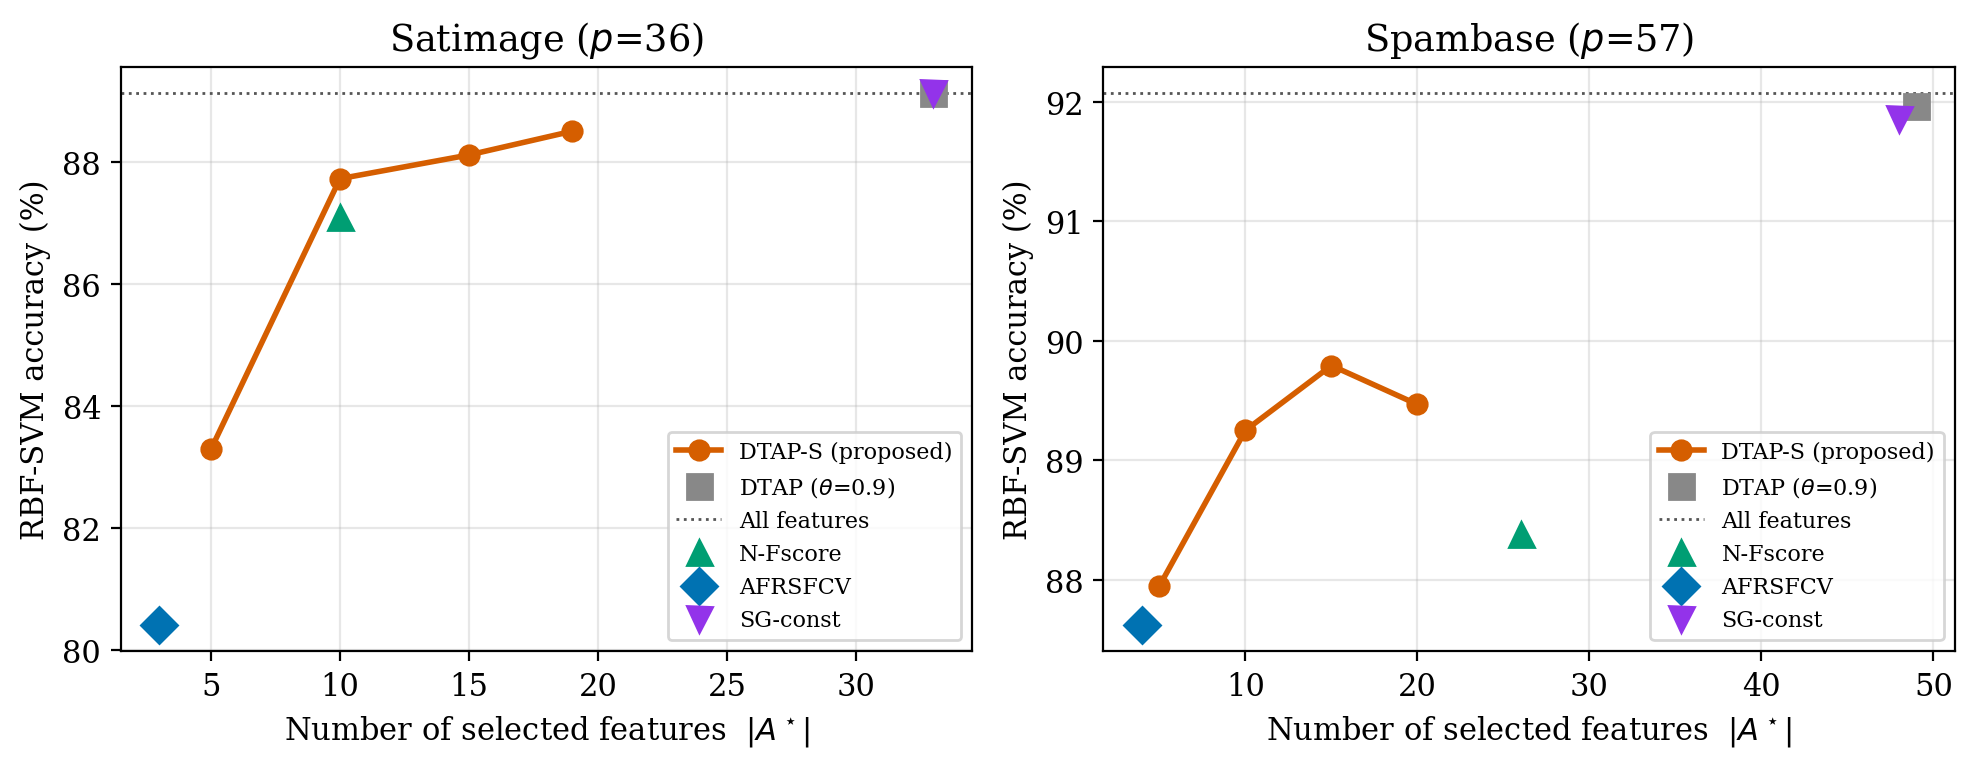
\includegraphics[width=\textwidth]{fig_acc_budget.png}
\caption{RBF-SVM accuracy versus selected size $|A^\star|$ on Satimage and Spambase. At similar selected sizes the \dtap-S curve (orange) lies above the baseline points, and on Spambase \dtap-S$_{10}$ outperforms N-Fscore with fewer features and higher accuracy.}\label{fig:dtaps}
\end{figure}

On Satimage and Spambase, where a small set of useful features exists, \dtap-S makes \dtap{} select a genuinely small set and outperforms the baselines at similar budgets. On Spambase, \dtap-S$_{10}$ uses only $10$ features yet reaches $89.25/88.71$ (SVM/$5$-NN) with perfect stability $\Phi=1.000$, while N-Fscore needs $26$ features for the lower $88.38/85.78$ at $\Phi=0.918$. \dtap-S$_{5}$ with $5$ features likewise outperforms AFRSFCV with $4$ features on all three measures. On Satimage at a matched $10$ features, \dtap-S$_{10}$ ($87.72/89.43$) again exceeds N-Fscore ($87.10/87.80$). The budget also cuts \dtap's own selection from $33$/$49$ features to $10$ while \emph{raising} stability from $0.595/0.846$ to $0.852/1.000$, since a fixed budget forces a consistent set across folds (Fig.~\ref{fig:dtaps}).

\subsection{Runtime and convergence}\label{ssec:runtime}
We now compare the computational cost and convergence behaviour of the five methods. Table~\ref{tab:runtime-summary} reports the wall-clock time, iteration count, and per-iteration cost of each method, averaged first over the cross-validation folds and then over the eight datasets; the per-dataset values are given in Appendix~\ref{app:exp-details} (Table~\ref{tab:runtime}).

\begin{table}[htbp]
\centering\small
\caption{Wall-clock time, iteration count, and per-iteration cost, averaged over the eight datasets (fold averages per dataset). The time averages are dominated by the largest datasets; per-dataset values are in Appendix~\ref{app:exp-details} (Table~\ref{tab:runtime}). Best per column in bold.}\label{tab:runtime-summary}
\begin{tabular}{l rrr}
\toprule
Method   & Time (s)         & Iterations      & Cost (ms/iter)   \\
\midrule
N-Fscore & $0.057$          & $999.0$         & $\mathbf{0.057}$ \\
AFRSFCV  & $1.620$          & $1000.0$        & $1.620$          \\
SG-const & $0.180$          & $300.7$         & $1.758$          \\
SG-dyn   & $0.883$          & $484.8$         & $25.569$         \\
DTAP     & $\mathbf{0.007}$ & $\mathbf{25.1}$ & $0.935$          \\
\bottomrule
\end{tabular}
\end{table}

Table~\ref{tab:runtime-summary} shows that \dtap{} has the lowest runtime, and the per-dataset values in Table~\ref{tab:runtime} confirm this on every one of the eight datasets. The advantage does not come from the per-iteration cost. As noted in Remark~\ref{rem:fs-cost}, \dtap, AFRSFCV, and SG-const share the same $O(nrp+p^2)$ per-iteration order, since all three compute the constraint gradients on the same input matrices. On Satimage, for instance, they measure $2.587$, $4.140$, and $4.492$ ms per iteration. The advantage comes from the iteration count. Thanks to the stopping test $J(w^k)\le\varepsilon$, \dtap{} stops after very few iterations, whereas AFRSFCV uses the full $1\,000$-iteration budget and SG-dyn often reaches it too. The gap is largest on the large sets. On Pendigits \dtap{} needs $0.004$ s versus $4.893$ s for AFRSFCV and $1.761$ s for SG-dyn, and on Satimage the three are $0.005$, $4.140$, and $2.032$ s. N-Fscore runs $999$ low-cost Euler steps that do not recompute the residual on large matrices, but it is still slower than \dtap{} on all eight sets.

A separate convergence experiment on the full data of each set gives a consistent picture (Fig.~\ref{fig:conv}). \dtap{} and SG-const drive $J$ below $\varepsilon$ on all eight datasets, whereas SG-dyn reaches feasibility on only five. The reason is that the estimated H\"older modulus is often very large, about $6.5\times10^3$ on Segmentation for instance, which makes the dynamic step tiny and convergence slow. This agrees with Theorem~\ref{thm:strong} on the strong convergence of \dtap{} and shows the benefit of the Polyak step on the convex track. \dtap{} avoids estimating the H\"older modulus and still reaches feasibility in few iterations.

\begin{figure}[H]
\centering
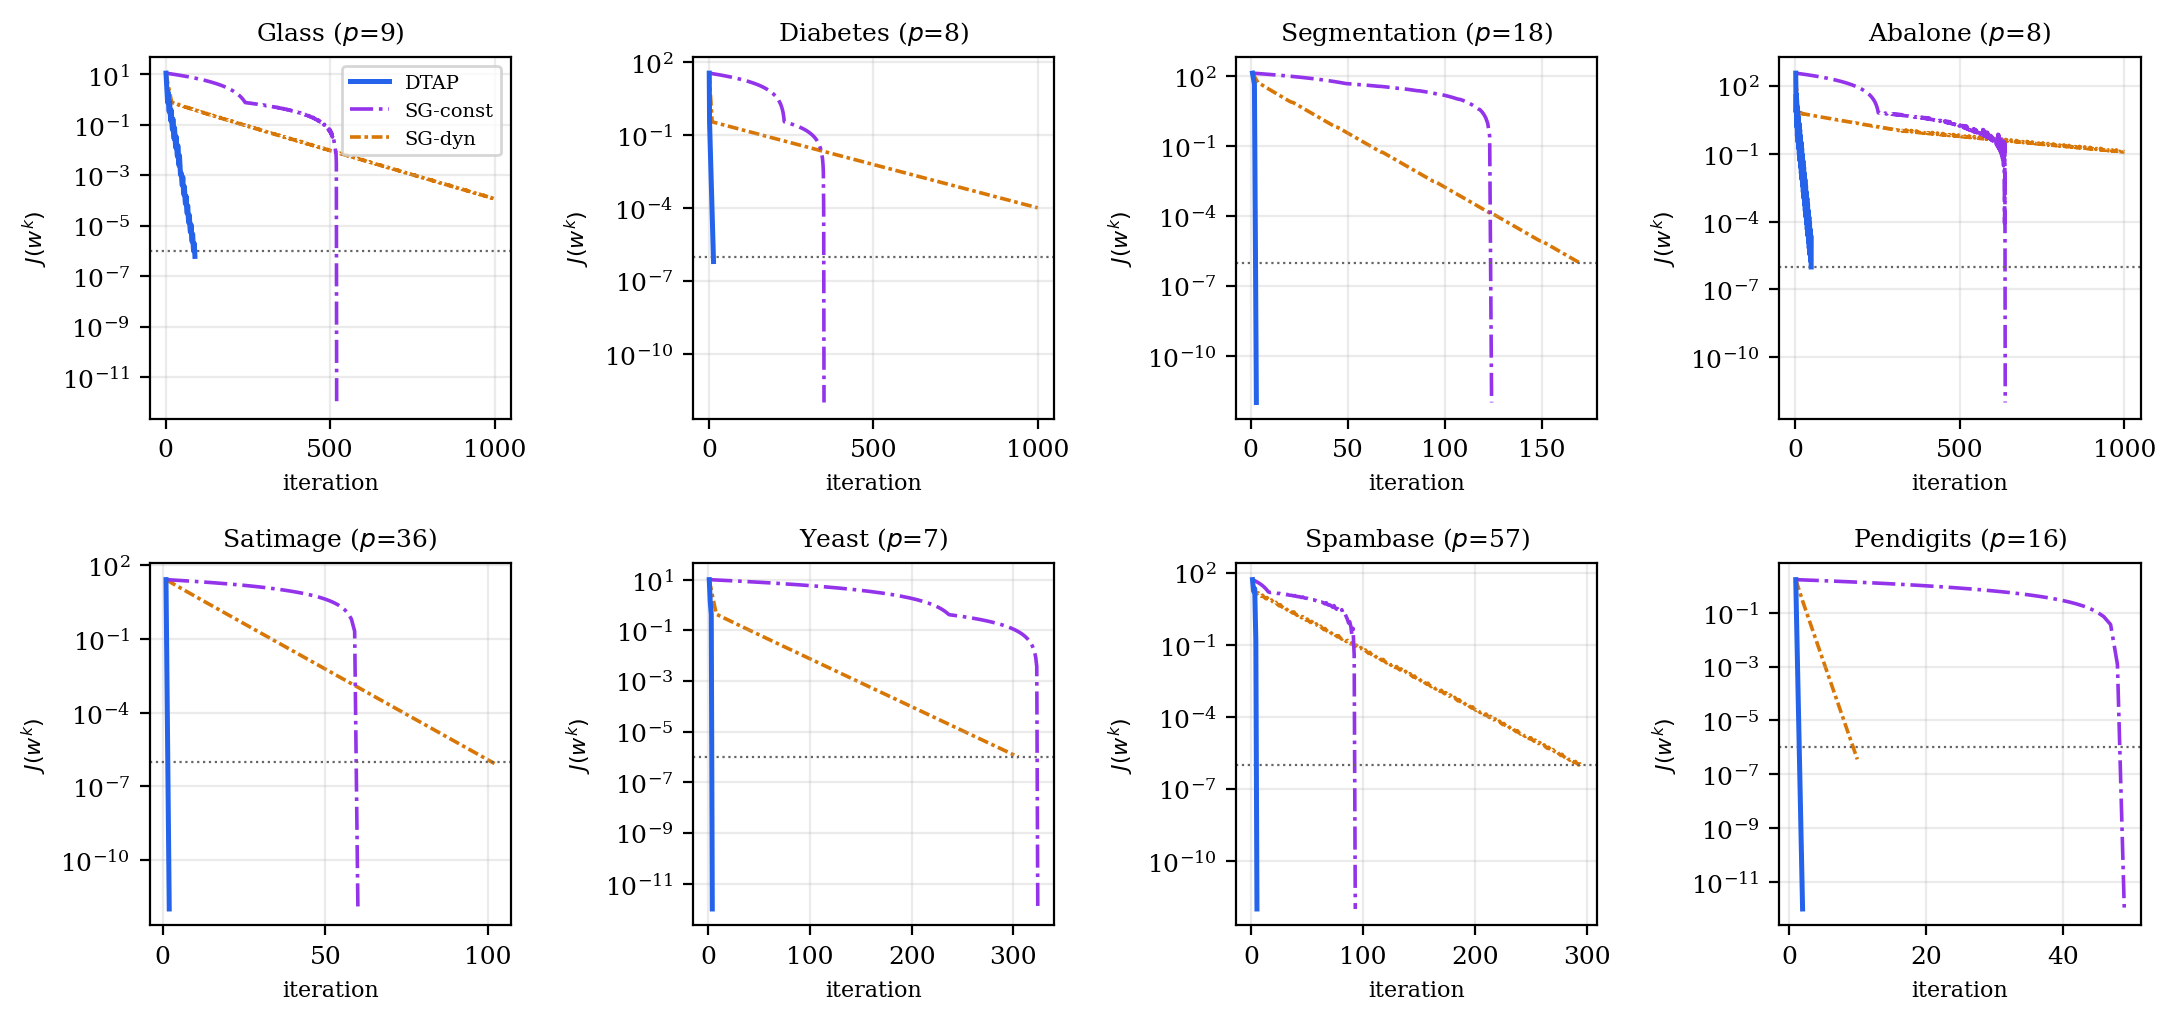
\includegraphics[width=\textwidth]{q2_convergence_overlay.png}
\caption{Violation $J(w^k)$ (log scale) versus iteration for \dtap, SG-const, and SG-dyn on the eight datasets. \dtap{} (solid) reaches feasibility in very few iterations on every dataset, while SG-dyn (dashed) stalls on several because the estimated H\"older modulus makes its step size too small.}\label{fig:conv}
\end{figure}

\subsection{Further analyses of robustness, fidelity, and ablation}\label{ssec:further}
Five additional experiments examine the reasons behind the results above; we summarise them briefly. \emph{(i) Constant-free robustness.} Every subgradient baseline must fix a step constant, namely $v$ for SG-const and the H\"older modulus $L$ for SG-dyn, and it reaches feasibility only inside a narrow band of that constant. Averaged over five datasets and nine swept values, SG-const succeeds for $6.2/9$ values and SG-dyn for $3.8/9$, whereas \dtap{} carries no such constant and reaches feasibility from the single standard start on all eight datasets. \emph{(ii) Deterministic convergence.} From the standard start \dtap{} reaches $J\le\varepsilon$ on all eight sets, SG-const does so as well but with $5$--$81\times$ more iterations, and SG-dyn succeeds on only five because it stalls when the estimated modulus shrinks its step. The \dtap{} trajectory also has no run-to-run variance. \emph{(iii) Performance profile.} On iteration count \dtap{} is fastest on all eight datasets ($\rho(1)=1.0$), which confirms that the speed-up of Section~\ref{ssec:runtime} comes from the iteration count, not the per-iteration cost. \emph{(iv) Selection fidelity on synthetic ground truth.} On controlled data ($n{=}600$, $p{=}30$, four classes, eight informative features), \dtap{} recovers all informative features at every redundancy level, rejects the most noise, and reaches the highest precision of the three selection methods, whereas the N-Fscore PNN under-selects and discards $12$--$44\%$ of the informative features. \emph{(v) Dual-track ablation.} Collapsing \dtap{} to a single track supports the design. A single diminishing-step subgradient on all constraints fails to reach feasibility within budget on four of five datasets, and a Polyak-only variant has no guarantee once the pseudoconvex constraint binds; only the full dual-track scheme is both guaranteed and fast. A Nemenyi critical-difference test on SVM accuracy ranks \dtap{} first (mean rank $2.17$), significantly ahead of AFRSFCV.

\subsection{Summary of findings}\label{ssec:exp-summary}
The numerical study supports four conclusions. (i) \emph{Quality.} \dtap{} matches or exceeds the full-feature accuracy and AUC on most datasets and outperforms both base models on the SVM metrics (Tables~\ref{tab:perf-summary} and~\ref{tab:wilcoxon}). (ii) \emph{Selection size.} The two convex constraints retain enough features to preserve the multi-class structure, in contrast to the overly sparse softmax selections of AFRSFCV (Table~\ref{tab:nfeat}). (iii) \emph{Speed.} \dtap{} is the fastest method on all eight datasets, by up to three orders of magnitude on the large sets, and the gain comes from the iteration count rather than the per-iteration cost (Table~\ref{tab:runtime-summary}). (iv) \emph{Robust convergence.} \dtap{} reaches feasibility on all eight datasets, whereas SG-dyn does so on only five because its H\"older-modulus estimate makes the step size too small (Fig.~\ref{fig:conv}). Finally, \dtap{} and the Hu variants give nearly identical selections (Wilcoxon $p=1$ on three of the four metrics, with only a small difference on RBF-SVM AUC), so the split-feasibility formulation delivers the quality, while the \dtap{} design delivers the speed.



\section{Conclusion}\label{sec:conclusion}
We studied a nonlinear split feasibility problem with a normal-box output set and mixed convex--pseudoconvex component maps. A Tchebyshev scalarization reduced feasibility to a closed-form max-type violation function, and we proposed \dtap, a dual-track algorithm that takes a residual-adaptive step on the convex constraints and a safeguarded diminishing step on the pseudoconvex ones, fuses the two by a soft weight, and projects only onto the base set. On the convex track the step is the constant-free rule of L\'opez et al.~\citep{lopez2012} extended to the nonlinear setting, licensed now by convexity of the individual components rather than by firm nonexpansiveness of a linear composition; the pseudoconvex track absorbs the remaining constraints on the sign that pseudoconvexity still supplies. Its step sizes need no operator-norm, Lipschitz, or H\"older constant, and we proved strong convergence to a feasible point (Theorem~\ref{thm:strong}). Two predecessors are closest. Against the nonlinear multiple-sets solver of Li et al.~\citep{li2013nsfp}, \dtap{} uses the same search direction but replaces the global, unverifiable hypothesis that the aggregate proximity function be convex (a hypothesis that a single pseudoconvex component invalidates, leaving the backtracking search possibly undefined) by a per-constraint classification and a closed-form step, and it drops the boundedness and global-Lipschitz requirements of that analysis. Against the subgradient method of Yen et al.~\citep{yen2019}, with which it shares the max-type scalarization and the active-set Clarke direction, \dtap{} differs in the admissible class (convex-plus-pseudoconvex, which neither contains nor is contained in their quasilinear class) and in driving the convex part by a non-diminishing, residual-scaled step rather than a prescribed diminishing sequence (Table~\ref{tab:related}).

On the application side, two previously separate feature-selection models reduce to a single normal-box NSFP whose constraints are drawn from their objectives, and the sparse variant \dtap-S adds an explicit feature budget. On eight UCI benchmarks \dtap{} preserved or improved accuracy and AUC over the base models, with the clearest gains on the SVM metrics, and reached feasibility substantially faster than the same-class subgradient methods, while \dtap-S gave compact, stable selections that outperform the baselines at matched size. This answers the three questions posed in the introduction.

Several limitations should be stated plainly. The theory delivers a feasibility guarantee rather than optimality, with a worst-case best-violation rate of $O(N^{-1/3})$ (Remark~\ref{rem:rate}), and sharper rates need extra structure such as an error bound. Performance depends on the threshold calibration of Section~\ref{sssec:thresholds}, since the percentiles are tuned per dataset and a poor choice can empty $\Omega$; the calibration is applied identically to the whole split-feasibility group, so it cannot favour \dtap{} over its same-class competitors. The iteration count can grow with the feature dimension, and the $p\gg n$ regime of text or genomic data is untested. Finally, we report two classifiers and two metrics on eight datasets, a modest sample, so we treat marginal tests such as the $5$-NN AUC as inconclusive.

Because criteria enter the model as constraints, further objectives such as sparsity surrogates or fairness penalties can be appended as convex or pseudoconvex constraints without changing the solver. An inertial acceleration would control the asymptotic regularity of Proposition~\ref{prop:regularity}, and the Hilbert-space analysis points to infinite-dimensional extensions and to other applications of nonlinear split feasibility, such as equilibrium models~\citep{yen2019} and constrained learning~\citep{tuan2024}.

\section*{Declaration of competing interest}
The authors declare that they have no known competing financial interests or
personal relationships that could have appeared to influence the work reported
in this paper.

\section*{Funding}
The authors received no specific funding for this work.

\section*{Declaration of generative AI use}
The authors report that generative AI was not used in the research or the
preparation of this manuscript.

\section*{Data availability}
The eight datasets used in this study are publicly available from the UCI Machine
Learning Repository~\citep{kelly2023uci}. An implementation of \dtap{} and the
baseline solvers is available from the authors on reasonable request.

\section*{ORCID}
\noindent Nguyen Van The~\raisebox{-0.1ex}{\textit{https://orcid.org/0009-0004-6548-420X}}\\
Tran Ngoc Thang~\raisebox{-0.1ex}{\textit{https://orcid.org/0009-0000-9549-5736}}\\
Nguyen Hong Son~\raisebox{-0.1ex}{\textit{https://orcid.org/0009-0006-3106-8296}}

\begin{thebibliography}{99}
\providecommand{\natexlab}[1]{#1}
\providecommand{\url}[1]{\texttt{#1}}
\expandafter\ifx\csname urlstyle\endcsname\relax
  \providecommand{\doi}[1]{doi: #1}\else
  \providecommand{\doi}{doi: \begingroup \urlstyle{rm}\Url}\fi

\bibitem[Bauschke and Borwein(1996)]{bauschkeborwein1996}
H.~H. Bauschke and J.~M. Borwein.
\newblock On projection algorithms for solving convex feasibility problems.
\newblock \emph{SIAM Review}, 38\penalty0 (3):\penalty0 367--426, 1996.
\newblock \doi{10.1137/S0036144593251710}.

\bibitem[Bauschke and Combettes(2011)]{bauschke2011}
H.~H. Bauschke and P.~L. Combettes.
\newblock \emph{Convex Analysis and Monotone Operator Theory in {H}ilbert Spaces}.
\newblock CMS Books in Mathematics. Springer, New York, 2011.
\newblock \doi{10.1007/978-1-4419-9467-7}.

\bibitem[Boyd et~al.(2011)Boyd, Parikh, Chu, Peleato, and Eckstein]{boyd2011admm}
Stephen Boyd, Neal Parikh, Eric Chu, Borja Peleato, and Jonathan Eckstein.
\newblock Distributed optimization and statistical learning via the alternating direction method of multipliers.
\newblock \emph{Foundations and Trends in Machine Learning}, 3\penalty0 (1):\penalty0 1--122, 2011.
\newblock \doi{10.1561/2200000016}.

\bibitem[Brown et~al.(2012)Brown, Pocock, Zhao, and Luj{\'a}n]{brown2012}
Gavin Brown, Adam Pocock, Ming-Jie Zhao, and Mikel Luj{\'a}n.
\newblock Conditional likelihood maximization: a unifying framework for information theoretic feature selection.
\newblock \emph{Journal of Machine Learning Research}, 13:\penalty0 27--66, 2012.

\bibitem[Byrne(2002)]{byrne2002}
C.~Byrne.
\newblock Iterative oblique projection onto convex sets and the split feasibility problem.
\newblock \emph{Inverse Problems}, 18\penalty0 (2):\penalty0 441--453, 2002.
\newblock \doi{10.1088/0266-5611/18/2/310}.

\bibitem[Censor and Elfving(1994)]{censor1994}
Y.~Censor and T.~Elfving.
\newblock A multiprojection algorithm using {B}regman projections in a product space.
\newblock \emph{Numerical Algorithms}, 8:\penalty0 221--239, 1994.
\newblock \doi{10.1007/BF02142692}.

\bibitem[Censor et~al.(2006)Censor, Bortfeld, Martin, and Trofimov]{censor2006}
Y.~Censor, T.~Bortfeld, B.~Martin, and A.~Trofimov.
\newblock A unified approach for inversion problems in intensity-modulated radiation therapy.
\newblock \emph{Physics in Medicine and Biology}, 51\penalty0 (10):\penalty0 2353--2365, 2006.
\newblock \doi{10.1088/0031-9155/51/10/001}.

\bibitem[Chen et~al.(2019)Chen, Postolache, and Yao]{chen2019ssub}
J.~Chen, M.~Postolache, and Y.~Yao.
\newblock S-subgradient projection methods with S-subdifferential functions for nonconvex split feasibility problems.
\newblock \emph{Symmetry}, 11\penalty0 (12):\penalty0 1517, 2019.
\newblock \doi{10.3390/sym11121517}.

\bibitem[Combettes and Pesquet(2011)]{combettes2011}
P.~L. Combettes and J.-C. Pesquet.
\newblock Proximal splitting methods in signal processing.
\newblock In \emph{Fixed-Point Algorithms for Inverse Problems in Science and Engineering}, pages 185--212. Springer, New York, 2011.
\newblock \doi{10.1007/978-1-4419-9569-8_10}.

\bibitem[Combettes(2001)]{combettes2001quasifejer}
Patrick~L. Combettes.
\newblock Quasi-fej{\'e}rian analysis of some optimization algorithms.
\newblock In D.~Butnariu, Y.~Censor, and S.~Reich, editors, \emph{Inherently Parallel Algorithms in Feasibility and Optimization and Their Applications}, volume~8 of \emph{Studies in Computational Mathematics}, pages 115--152. Elsevier, Amsterdam, 2001.
\newblock \doi{10.1016/S1570-579X(01)80010-0}.

\bibitem[Condat(2016)]{condat2016simplex}
Laurent Condat.
\newblock Fast projection onto the simplex and the $\ell_1$ ball.
\newblock \emph{Mathematical Programming}, 158\penalty0 (1):\penalty0 575--585, 2016.
\newblock \doi{10.1007/s10107-015-0946-6}.

\bibitem[Cortes and Vapnik(1995)]{cortes1995svm}
Corinna Cortes and Vladimir Vapnik.
\newblock Support-vector networks.
\newblock \emph{Machine Learning}, 20\penalty0 (3):\penalty0 273--297, 1995.
\newblock \doi{10.1007/BF00994018}.

\bibitem[Cover and Hart(1967)]{cover1967knn}
Thomas~M. Cover and Peter~E. Hart.
\newblock Nearest neighbour pattern classification.
\newblock \emph{IEEE Transactions on Information Theory}, 13\penalty0 (1):\penalty0 21--27, 1967.
\newblock \doi{10.1109/TIT.1967.1053964}.

\bibitem[Dem{\v{s}}ar(2006)]{demsar2006}
Janez Dem{\v{s}}ar.
\newblock Statistical comparisons of classifiers over multiple data sets.
\newblock \emph{Journal of Machine Learning Research}, 7:\penalty0 1--30, 2006.
\newblock URL \url{https://jmlr.org/papers/v7/demsar06a.html}.

\bibitem[Fukushima(1986)]{fukushima1986}
M.~Fukushima.
\newblock A relaxed projection method for variational inequalities.
\newblock \emph{Mathematical Programming}, 35\penalty0 (1):\penalty0 58--70, 1986.
\newblock \doi{10.1007/BF01589441}.

\bibitem[Guyon and Elisseeff(2003)]{guyon2003}
Isabelle Guyon and Andr{\'e} Elisseeff.
\newblock An introduction to variable and feature selection.
\newblock \emph{Journal of Machine Learning Research}, 3:\penalty0 1157--1182, 2003.

\bibitem[Hand and Till(2001)]{handtill2001}
David~J. Hand and Robert~J. Till.
\newblock A simple generalization of the area under the {ROC} curve for multiple class classification problems.
\newblock \emph{Machine Learning}, 45\penalty0 (2):\penalty0 171--186, 2001.
\newblock \doi{10.1023/A:1010920819831}.

\bibitem[Hoang(2016)]{hoang2016}
Tuy Hoang.
\newblock \emph{Convex Analysis and Global Optimization}.
\newblock Springer International Publishing, Switzerland, 2nd edition, 2016.
\newblock \doi{10.1007/978-3-319-31484-6}.

\bibitem[Hu et~al.(2022)Hu, Li, Yu, and Yip]{hu2022quasi}
Y.~Hu, G.~Li, C.~K.~W. Yu, and T.~L. Yip.
\newblock Quasi-convex feasibility problems: Subgradient methods and convergence rates.
\newblock \emph{European Journal of Operational Research}, 298\penalty0 (1):\penalty0 45--58, 2022.
\newblock \doi{10.1016/j.ejor.2021.09.029}.

\bibitem[Jensen and Shen(2009)]{jensen2009}
Richard Jensen and Qiang Shen.
\newblock New approaches to fuzzy-rough feature selection.
\newblock \emph{IEEE Transactions on Fuzzy Systems}, 17\penalty0 (4):\penalty0 824--838, 2009.
\newblock \doi{10.1109/TFUZZ.2008.924209}.

\bibitem[Kelly et~al.(2023)Kelly, Longjohn, and Nottingham]{kelly2023uci}
Markelle Kelly, Rachel Longjohn, and Kolby Nottingham.
\newblock The {UCI} machine learning repository.
\newblock \url{https://archive.ics.uci.edu}, 2023.
\newblock Accessed 2026.

\bibitem[Kyrillidis et~al.(2013)Kyrillidis, Becker, Cevher, and Koch]{kyrillidis2013}
Anastasios Kyrillidis, Stephen Becker, Volkan Cevher, and Christoph Koch.
\newblock Sparse projections onto the simplex.
\newblock In \emph{Proceedings of the 30th International Conference on Machine Learning (ICML)}, volume~28 of \emph{PMLR}, pages 235--243, 2013.

\bibitem[Li et~al.(2013)Li, Han, and Zhang]{li2013nsfp}
Z.~Li, D.~Han, and W.~Zhang.
\newblock A self-adaptive projection-type method for nonlinear multiple-sets split feasibility problem.
\newblock \emph{Inverse Problems in Science and Engineering}, 21\penalty0 (1):\penalty0 155--170, 2013.
\newblock \doi{10.1080/17415977.2012.677445}.

\bibitem[Liu et~al.(2026)Liu, Yang, Ding, Ju, Li, Wang, and Yin]{liu2026rfs}
Keyu Liu, Xibei Yang, Weiping Ding, Hengrong Ju, Tianrui Li, Jie Wang, and Tengyu Yin.
\newblock A survey on rough feature selection: Recent advances and challenges.
\newblock \emph{{IEEE}/{CAA} Journal of Automatica Sinica}, 13\penalty0 (3):\penalty0 521--542, 2026.
\newblock \doi{10.1109/JAS.2025.125231}.

\bibitem[L{\'o}pez et~al.(2012)L{\'o}pez, Mart{\'\i}n-M{\'a}rquez, Wang, and Xu]{lopez2012}
G.~L{\'o}pez, V.~Mart{\'\i}n-M{\'a}rquez, F.~Wang, and H.-K. Xu.
\newblock Solving the split feasibility problem without prior knowledge of matrix norms.
\newblock \emph{Inverse Problems}, 28\penalty0 (8):\penalty0 085004, 2012.
\newblock \doi{10.1088/0266-5611/28/8/085004}.

\bibitem[Mangasarian(1965)]{mangasarian1965}
O.~L. Mangasarian.
\newblock Pseudo-convex functions.
\newblock \emph{SIAM Journal on Control}, 3\penalty0 (2):\penalty0 281--290, 1965.
\newblock \doi{10.1137/0303020}.

\bibitem[Mangasarian(1994)]{mangasarian1994}
O.~L. Mangasarian.
\newblock \emph{Nonlinear Programming}.
\newblock Classics in Applied Mathematics. SIAM, Philadelphia, 1994.
\newblock \doi{10.1137/1.9781611971255}.

\bibitem[Nogueira et~al.(2018)Nogueira, Sechidis, and Brown]{nogueira2018}
Sarah Nogueira, Konstantinos Sechidis, and Gavin Brown.
\newblock On the stability of feature selection algorithms.
\newblock \emph{Journal of Machine Learning Research}, 18\penalty0 (174):\penalty0 1--54, 2018.

\bibitem[Polyak(1969)]{polyak1969}
B.~T. Polyak.
\newblock Minimization of unsmooth functionals.
\newblock \emph{USSR Computational Mathematics and Mathematical Physics}, 9\penalty0 (3):\penalty0 14--29, 1969.
\newblock \doi{10.1016/0041-5553(69)90061-5}.

\bibitem[Theng and Bhoyar(2024)]{theng2024fs}
Dipti Theng and Kishor~K. Bhoyar.
\newblock Feature selection techniques for machine learning: a survey of more than two decades of research.
\newblock \emph{Knowledge and Information Systems}, 66:\penalty0 1575--1637, 2024.
\newblock \doi{10.1007/s10115-023-02010-5}.

\bibitem[Tuan et~al.(2024)Tuan, Dung, and Thang]{tuan2024}
Tran~Anh Tuan, Nguyen~Viet Dung, and Tran~Ngoc Thang.
\newblock A hyper-transformer model for controllable pareto front learning with split feasibility constraints.
\newblock \emph{Neural Networks}, 179:\penalty0 106571, 2024.
\newblock \doi{10.1016/j.neunet.2024.106571}.

\bibitem[Wang et~al.(2021)Wang, Li, and Wang]{wang2021fractional}
Y.~Wang, X.~Li, and J.~Wang.
\newblock A neurodynamic optimization approach to supervised feature selection via fractional programming.
\newblock \emph{Neural Networks}, 136:\penalty0 194--206, 2021.
\newblock \doi{10.1016/j.neunet.2021.01.004}.

\bibitem[Wang et~al.(2026)Wang, Zhang, An, and Deng]{wang2026afrsfcv}
C.~Wang, Y.~Zhang, S.~An, and T.~Deng.
\newblock Adaptive feature selection based on fuzzy rough set fusion model with class variance.
\newblock \emph{Pattern Recognition}, 170:\penalty0 112014, 2026.
\newblock \doi{10.1016/j.patcog.2025.112014}.

\bibitem[Xu(2010)]{xu2010}
H.-K. Xu.
\newblock Iterative methods for the split feasibility problem in infinite-dimensional {H}ilbert spaces.
\newblock \emph{Inverse Problems}, 26\penalty0 (10):\penalty0 105018, 2010.
\newblock \doi{10.1088/0266-5611/26/10/105018}.

\bibitem[Yang(2004)]{yang2004}
Q.~Yang.
\newblock The relaxed {CQ} algorithm solving the split feasibility problem.
\newblock \emph{Inverse Problems}, 20\penalty0 (4):\penalty0 1261--1266, 2004.
\newblock \doi{10.1088/0266-5611/20/4/014}.

\bibitem[Yen et~al.(2019)Yen, Huyen, and Muu]{yen2019}
Le~Hai Yen, Nguyen Thi~Thanh Huyen, and Le~Dung Muu.
\newblock A subgradient algorithm for a class of nonlinear split feasibility problems: application to jointly constrained nash equilibrium models.
\newblock \emph{Journal of Global Optimization}, 73:\penalty0 849--868, 2019.
\newblock \doi{10.1007/s10898-018-00735-0}.

\end{thebibliography}


\appendix

\section{Baseline solvers}\label{app:baselines}
This appendix records the solver mechanics of the two base models, deferred from Sections~\ref{sssec:nfscore} and~\ref{sssec:afrsfcv-model} for readability.

\paragraph*{N-Fscore: the projection neural network}
To solve the fractional program~\eqref{eq:wangOrig}, Wang et al.~\citep{wang2021fractional} proposed a neurodynamic method coupling a projection neural network (PNN) with a $k$-winners-take-all network. The PNN is the differential system
\begin{equation}\label{eq:pnn}
\varepsilon_{\mathrm{PNN}}\frac{du}{dt}=-Pg(u)-(I-P)\bigl(u-g(u)+\nabla f((I-P)g(u)+\tfrac1p\mathbf{1}_p)\bigr)+\tfrac1p\mathbf{1}_p,
\end{equation}
with output $w=g(u)$, where $g(u)=\max\{0,u\}$ is the componentwise ReLU, $P=\tfrac1p\mathbf{1}_p\mathbf{1}_p^{\top}$, $\nabla f$ is the gradient of the objective in~\eqref{eq:wangOrig}, and $\varepsilon_{\mathrm{PNN}}>0$ is a time constant. We integrate~\eqref{eq:pnn} by explicit Euler on $[0,T]$ with $N_{\mathrm{step}}$ steps under a fixed budget (no stopping rule), with $T,N_{\mathrm{step}}$ large enough for $w$ to stabilize. For a uniform comparison we use only the PNN part to obtain $w^\star$; the $k$-WTA stage is replaced by the shared cumulative-threshold rule of Section~\ref{ssec:selection}.

\paragraph*{AFRSFCV: gradient and update}
The softmax loss~\eqref{eq:afrsfcvLoss} is minimized over $\tau\in\R^p$ by gradient descent. Its gradient is
\begin{equation}\label{eq:gradTau}
\nabla_\tau L(\tau)=\bigl(\diag(w(\tau))-w(\tau)w(\tau)^{\top}\bigr)\nabla_w L(w(\tau)),
\end{equation}
with $\nabla_w L=-\mathbf{M}^{\top}(\vecop(Y)-\mathbf{M}w)+\lambda_1(P^{\top}Pw-P^{\top}\mathbf{1}_n)+\lambda_2 w$, where $\mathbf{M}\in\R^{nr\times p}$ has $k$-th column $\vecop(\underline{R_k}(D))$. The update $\tau^{t+1}=\tau^t-\eta\,\nabla_\tau L(\tau^t)$ runs for a fixed budget of $T$ steps; the final weight $w^\star=w(\tau^T)\in K$ feeds the shared selection rule of Section~\ref{ssec:selection}.


\section{Experimental details}\label{app:exp-details}
This appendix collects the threshold calibration, the implementation details, and the per-dataset classification and runtime results deferred from Section~\ref{sec:experiments}.

\paragraph*{Output-threshold calibration}
For each dataset we evaluate $F_1,F_2,F_3$ at the $3\,000$ sampled points $w^{(s)}\sim\mathrm{Dir}(\mathbf{1}_p)$ and set $b_i$ to the $p_i$-th percentile of the resulting values, so about $p_i\%$ of simplex points satisfy $F_i\le b_i$ and the percentile controls the size of the feasible set. The percentiles $p_i$ are tuned per dataset (by sample size, dimension, class count, and balance). The resulting $b_i$, averaged over folds, appear in Table~\ref{tab:thresholds}.
\begin{table}[htbp]
\centering
\caption{Output thresholds $b_1,b_2,b_3$ (fold averages) per dataset.}\label{tab:thresholds}
\begin{tabular}{lrrr}
\toprule
Dataset      & $b_1$    & $b_2$    & $b_3$     \\
\midrule
Glass        & $142$    & $18.3$   & $0.0638$  \\
Diabetes     & $549$    & $98.9$   & $0.0443$  \\
Segmentation & $1\,450$ & $466$    & $0.00956$ \\
Abalone      & $2\,990$ & $1\,080$ & $0.105$   \\
Satimage     & $4\,570$ & $3\,200$ & $0.0356$  \\
Yeast        & $887$    & $579$    & $0.0524$  \\
Spambase     & $3\,250$ & $1\,010$ & $0.0800$  \\
Pendigits    & $7\,910$ & $7\,080$ & $0.0141$  \\
\bottomrule
\end{tabular}
\end{table}

\paragraph*{Implementation and reproducibility}
All five methods share one per-fold pipeline and consume identical precomputed inputs ($\underline{R_k}(D),P,Y,Q,\rho$). Min--max scaling is fit on each fold's training portion only, multi-information uses $10$-bin equal-width histograms~\citep{brown2012}, $Q$ is shifted by $\delta_Q=-\min\{0,\lambda_{\min}(S)\}$ to keep $Q\succeq0$, the Fisher denominator uses $\varepsilon_\rho=10^{-8}$, and the simplex projection is the sort-based $O(p\log p)$ algorithm~\citep{condat2016simplex}. Random seeds for the CV splits and the Dirichlet sampling are fixed, so the study is reproducible. Reported runtimes are relative cross-method measurements and are not sensitive to hardware, because the per-iteration cost is dominated by the shared matrix operations.

\paragraph*{Per-dataset classification results}
Table~\ref{tab:acc} reports the per-dataset accuracy and macro one-vs-rest AUC that underlie the averages of Table~\ref{tab:perf-summary}.


{\small
\begin{longtable}{ll rr rr}
\caption{Per-dataset classification accuracy (\%) and macro one-vs-rest AUC on the
held-out test set for RBF-SVM and $5$-NN. The best among the three selection methods
(N-Fscore, AFRSFCV, DTAP) is in bold.}\label{tab:acc} \\
\toprule
\multirow{2}{*}{Dataset} & \multirow{2}{*}{Method} & \multicolumn{2}{c}{Accuracy (\%)} & \multicolumn{2}{c}{AUC} \\
\cmidrule(lr){3-4}\cmidrule(lr){5-6}
 & & RBF-SVM & $5$-NN & RBF-SVM & $5$-NN \\
\midrule
\endfirsthead
\multicolumn{6}{l}{\footnotesize Table~\ref{tab:acc} (continued).} \\
\toprule
\multirow{2}{*}{Dataset} & \multirow{2}{*}{Method} & \multicolumn{2}{c}{Accuracy (\%)} & \multicolumn{2}{c}{AUC} \\
\cmidrule(lr){3-4}\cmidrule(lr){5-6}
 & & RBF-SVM & $5$-NN & RBF-SVM & $5$-NN \\
\midrule
\endhead
\midrule
\multicolumn{6}{r}{\footnotesize\emph{continued on next page}} \\
\endfoot
\bottomrule
\endlastfoot
\multirow{4}{*}{Glass}        & Full     & $76.74$          & $72.09$          & $0.9250$          & $0.9097$          \\*
                              & N-Fscore & $69.77$          & $\mathbf{74.42}$ & $0.9023$          & $0.8933$          \\*
                              & AFRSFCV  & $\mathbf{72.09}$ & $69.77$          & $0.9078$          & $\mathbf{0.9371}$ \\*
                              & DTAP     & $\mathbf{72.09}$ & $69.77$          & $\mathbf{0.9144}$ & $\mathbf{0.9371}$ \\
\midrule
\multirow{4}{*}{Diabetes}     & Full     & $74.68$          & $71.43$          & $0.8089$          & $0.7356$          \\*
                              & N-Fscore & $71.43$          & $70.78$          & $0.7956$          & $0.7154$          \\*
                              & AFRSFCV  & $65.58$          & $67.53$          & $0.6617$          & $0.7145$          \\*
                              & DTAP     & $\mathbf{74.68}$ & $\mathbf{73.38}$ & $\mathbf{0.8098}$ & $\mathbf{0.7766}$ \\
\midrule
\multirow{4}{*}{Segmentation} & Full     & $93.29$          & $94.37$          & $0.9937$          & $0.9880$          \\*
                              & N-Fscore & $80.52$          & $87.01$          & $0.9712$          & $0.9801$          \\*
                              & AFRSFCV  & $78.79$          & $86.58$          & $0.9668$          & $0.9646$          \\*
                              & DTAP     & $\mathbf{93.29}$ & $\mathbf{94.59}$ & $\mathbf{0.9940}$ & $\mathbf{0.9897}$ \\
\midrule
\multirow{4}{*}{Abalone}      & Full     & $61.60$          & $59.81$          & $0.8102$          & $0.7742$          \\*
                              & N-Fscore & $61.36$          & $\mathbf{61.00}$ & $0.8065$          & $0.7605$          \\*
                              & AFRSFCV  & $62.56$          & $58.73$          & $0.8113$          & $\mathbf{0.7752}$ \\*
                              & DTAP     & $\mathbf{62.68}$ & $60.29$          & $\mathbf{0.8123}$ & $0.7695$          \\
\midrule
\multirow{4}{*}{Satimage}     & Full     & $89.12$          & $91.14$          & $0.9796$          & $0.9792$          \\*
                              & N-Fscore & $87.10$          & $87.80$          & $0.9755$          & $0.9705$          \\*
                              & AFRSFCV  & $80.42$          & $80.96$          & $0.9611$          & $0.9306$          \\*
                              & DTAP     & $\mathbf{89.12}$ & $\mathbf{91.22}$ & $\mathbf{0.9796}$ & $\mathbf{0.9766}$ \\
\midrule
\multirow{4}{*}{Yeast}        & Full     & $58.25$          & $51.52$          & $0.8480$          & $0.7667$          \\*
                              & N-Fscore & $\mathbf{58.92}$ & $\mathbf{51.52}$ & $0.8057$          & $\mathbf{0.7763}$ \\*
                              & AFRSFCV  & $57.91$          & $\mathbf{51.52}$ & $0.8218$          & $0.7681$          \\*
                              & DTAP     & $58.59$          & $\mathbf{51.52}$ & $\mathbf{0.8380}$ & $0.7585$          \\
\midrule
\multirow{4}{*}{Spambase}     & Full     & $92.07$          & $90.34$          & $0.9663$          & $0.9443$          \\*
                              & N-Fscore & $88.38$          & $85.78$          & $0.9391$          & $0.9214$          \\*
                              & AFRSFCV  & $87.62$          & $88.49$          & $0.9155$          & $0.9206$          \\*
                              & DTAP     & $\mathbf{91.97}$ & $\mathbf{89.25}$ & $\mathbf{0.9615}$ & $\mathbf{0.9437}$ \\
\midrule
\multirow{4}{*}{Pendigits}    & Full     & $99.09$          & $98.95$          & $0.9995$          & $0.9982$          \\*
                              & N-Fscore & $\mathbf{98.95}$ & $98.64$          & $\mathbf{0.9996}$ & $0.9982$          \\*
                              & AFRSFCV  & $97.77$          & $97.73$          & $\mathbf{0.9996}$ & $0.9965$          \\*
                              & DTAP     & $\mathbf{98.95}$ & $\mathbf{99.05}$ & $0.9995$          & $\mathbf{0.9987}$ \\
\end{longtable}
}

\paragraph*{Per-dataset runtime}
Table~\ref{tab:runtime} reports the per-dataset wall-clock time, iteration count, and per-iteration cost that underlie the averages of Table~\ref{tab:runtime-summary}.

{\footnotesize
\begin{longtable}{ll rrr}
\caption{Wall-clock time, iteration count, and per-iteration cost (fold averages)
of the five methods.}\label{tab:runtime} \\
\toprule
Dataset & Method & Time (s) & Iterations & Cost (ms/iter) \\
\midrule
\endfirsthead
\multicolumn{5}{l}{\footnotesize Table~\ref{tab:runtime} (continued).} \\
\toprule
Dataset & Method & Time (s) & Iterations & Cost (ms/iter) \\
\midrule
\endhead
\midrule
\multicolumn{5}{r}{\footnotesize\emph{continued on next page}} \\
\endfoot
\bottomrule
\endlastfoot
\multirow{5}{*}{Glass}        & N-Fscore & $0.059$          & $999.0$         & $\mathbf{0.059}$ \\*
                              & AFRSFCV  & $0.160$          & $1000.0$        & $0.160$          \\*
                              & SG-const & $0.101$          & $503.1$         & $0.201$          \\*
                              & SG-dyn   & $0.265$          & $991.4$         & $0.267$          \\*
                              & DTAP     & $\mathbf{0.012}$ & $\mathbf{75.7}$ & $0.148$          \\
\midrule
\multirow{5}{*}{Diabetes}     & N-Fscore & $0.057$          & $999.0$         & $\mathbf{0.057}$ \\*
                              & AFRSFCV  & $0.166$          & $1000.0$        & $0.166$          \\*
                              & SG-const & $0.070$          & $324.7$         & $0.216$          \\*
                              & SG-dyn   & $0.245$          & $923.6$         & $0.272$          \\*
                              & DTAP     & $\mathbf{0.002}$ & $\mathbf{11.7}$ & $0.169$          \\
\midrule
\multirow{5}{*}{Segmentation} & N-Fscore & $0.056$          & $999.0$         & $\mathbf{0.056}$ \\*
                              & AFRSFCV  & $0.712$          & $1000.0$        & $0.712$          \\*
                              & SG-const & $0.098$          & $124.5$         & $0.786$          \\*
                              & SG-dyn   & $0.341$          & $159.7$         & $2.133$          \\*
                              & DTAP     & $\mathbf{0.003}$ & $\mathbf{4.9}$  & $0.557$          \\
\midrule
\multirow{5}{*}{Abalone}      & N-Fscore & $0.055$          & $999.0$         & $\mathbf{0.055}$ \\*
                              & AFRSFCV  & $0.289$          & $1000.0$        & $0.289$          \\*
                              & SG-const & $0.284$          & $881.8$         & $0.322$          \\*
                              & SG-dyn   & $0.415$          & $1000.0$        & $0.415$          \\*
                              & DTAP     & $\mathbf{0.021}$ & $\mathbf{88.0}$ & $0.243$          \\
\midrule
\multirow{5}{*}{Satimage}     & N-Fscore & $0.058$          & $999.0$         & $\mathbf{0.058}$ \\*
                              & AFRSFCV  & $4.140$          & $1000.0$        & $4.140$          \\*
                              & SG-const & $0.274$          & $61.0$          & $4.492$          \\*
                              & SG-dyn   & $2.032$          & $107.0$         & $18.998$         \\*
                              & DTAP     & $\mathbf{0.005}$ & $\mathbf{2.0}$  & $2.587$          \\
\midrule
\multirow{5}{*}{Yeast}        & N-Fscore & $0.055$          & $999.0$         & $\mathbf{0.055}$ \\*
                              & AFRSFCV  & $0.240$          & $1000.0$        & $0.240$          \\*
                              & SG-const & $0.099$          & $365.0$         & $0.271$          \\*
                              & SG-dyn   & $0.180$          & $377.0$         & $0.501$          \\*
                              & DTAP     & $\mathbf{0.002}$ & $\mathbf{11.2}$ & $0.174$          \\
\midrule
\multirow{5}{*}{Spambase}     & N-Fscore & $0.063$          & $999.0$         & $\mathbf{0.063}$ \\*
                              & AFRSFCV  & $2.357$          & $1000.0$        & $2.357$          \\*
                              & SG-const & $0.265$          & $97.0$          & $2.730$          \\*
                              & SG-dyn   & $1.827$          & $309.8$         & $5.902$          \\*
                              & DTAP     & $\mathbf{0.008}$ & $\mathbf{5.0}$  & $1.513$          \\
\midrule
\multirow{5}{*}{Pendigits}    & N-Fscore & $0.056$          & $999.0$         & $\mathbf{0.056}$ \\*
                              & AFRSFCV  & $4.893$          & $1000.0$        & $4.893$          \\*
                              & SG-const & $0.246$          & $48.7$          & $5.043$          \\*
                              & SG-dyn   & $1.761$          & $10.0$          & $176.065$        \\*
                              & DTAP     & $\mathbf{0.004}$ & $\mathbf{2.0}$  & $2.086$          \\
\end{longtable}
}


\end{document}
